\documentclass[
       oneside,
       english,
       brazil
       ]{abntbibufjf}

\usepackage[T1]{fontenc}
\usepackage[utf8]{inputenc}
\usepackage{lmodern}
\usepackage{amsmath, xparse, amssymb}
\usepackage{lastpage}
\usepackage{indentfirst}
\usepackage{color}
\usepackage{graphicx}
\usepackage{microtype}
\usepackage{hyperref}
\usepackage{xurl}
\usepackage{float}
\usepackage{subcaption}
\usepackage{pdfpages}
\usepackage{booktabs}
\usepackage{tabularx}
\usepackage{multirow}
\usepackage{array}

%% -----------------------------------------------------------------------------

\titulo{Aprendizado de Máquina para Seleção de Pixels em Baixas Energias no Experimento~CYGNO}
\subtitulo{Proposta de Qualificação de Doutorado}
\autor{Guilherme Sebastião Pinheiro Lopes}
\autorVirg{Lopes, Guilherme Sebastião Pinheiro}
\local{Juiz de Fora}
\data{2025}
\orientador[Orientador:]{Rafael Antunes Nóbrega}
\coorientador[Coorientador:]{Igor Abritta Costa}
\orientadorTitulo{Prof. Dr.}
\coorientadorTitulo{Prof. Dr.}
\instituicao{Universidade Federal de Juiz de Fora}
\faculdade{Faculdade de Engenharia}
\programa{PROGRAMA DE PÓS-GRADUAÇÃO EM ENGENHARIA ELÉTRICA}
\objeto{Proposta de Qualificação (Doutorado)}
\natureza{Proposta de qualificação apresentada ao \insereprograma~da
Universidade Federal de Juiz de Fora como requisito parcial à obtenção do
título de Doutor em Engenharia Elétrica.
Área de concentração: Sistemas de Informação e Comunicação.
}

\finalcatalog{1. Aprendizado de Máquina. 2. CYGNO. 3. Matéria Escura.
4. Seleção de Pixels. I. Nóbrega, Rafael Antunes, orient.
II. Costa, Igor Abritta, coorient. III. Título.}

\usepackage[round, numbers]{natbib}

\begin{document}

%% ELEMENTOS PRÉ-TEXTUAIS

\inserecapa

\inserefolhaderosto

\inserecatalog

\begin{folhadeaprovacao}
\inicfolhaaprov

Aprovada em \underline{\hspace{1cm}} de \underline{\hspace{2.5cm}} de \underline{\hspace{1.2cm}}

\vfill
\begin{center} BANCA EXAMINADORA \end{center}

\assinatura{Prof. Dr. Rafael Antunes Nóbrega\ -- Orientador \\ Universidade Federal de Juiz de Fora}
\assinatura{Prof. Dr. Igor Abritta Costa\ -- Coorientador \\ Universidade Federal de Juiz de Fora}
\assinatura{Titulação Nome e Sobrenome \\ Instituição}
\assinatura{Titulação Nome e Sobrenome \\ Instituição}
\end{folhadeaprovacao}
\cleardoublepage


\begin{dedicatoria}
Aos meus pais e à minha família, pelo apoio incondicional em todos os momentos desta jornada.
\end{dedicatoria}


\begin{agradecimentos}
Agradeço ao meu orientador Prof.\ Dr.\ Rafael Antunes Nóbrega e ao meu
coorientador Prof.\ Dr.\ Igor Abritta Costa pelo suporte, pela orientação e
pela confiança depositada ao longo deste trabalho. À colaboração CYGNO, pelo
ambiente de pesquisa colaborativo, pelo acesso aos dados e pelas discussões
sempre enriquecedoras. Aos colegas do Programa de Pós-Graduação em Engenharia
Elétrica da UFJF, pela troca de conhecimentos e pelo companheirismo. Às
instituições INFN-Roma\,I, Gran Sasso Science Institute, Dipartimento di Fisica
della Sapienza Università di Roma, INFN-LNF e demais membros da colaboração
CYGNO, pelo trabalho conjunto que torna este experimento possível.
\end{agradecimentos}


\begin{epigrafemenos}
``A ciência é uma forma de pensar muito mais do que um conjunto de
conhecimentos.'' (SAGAN, Carl. \textit{O Mundo Assombrado pelos Demônios},
1995).
\end{epigrafemenos}


\begin{resumo}

Este trabalho apresenta o desenvolvimento de uma metodologia baseada em
aprendizado profundo para a etapa de seleção de pixels no algoritmo de
reconstrução do Experimento CYGNO, com foco especial em eventos de baixa
energia na faixa de 0,25 a 1~keV. O Experimento CYGNO é um detector de
projeção de tempo (TPC) com leitura óptica por câmera sCMOS, desenvolvido
para a detecção direta de matéria escura com massas na faixa de 1 a
10~GeV/c². Em trabalho anterior de mestrado, foi realizada uma comparação
sistemática entre filtros clássicos de processamento de imagens (filtros de
média, gaussiano e mediana) e uma rede neural U-Net aplicada à seleção de
pixels nas imagens do detector. Os resultados demonstraram a superioridade da
U-Net (F1-score: 0,873) em relação ao filtro de mediana (F1-score: 0,820) e
ao algoritmo original do experimento (F1-score: 0,137), motivando o
aprofundamento da investigação com foco em baixas energias ainda não
exploradas sistematicamente. O presente trabalho estende essa investigação
utilizando dados de simulação mais recentes cobrindo energias de 0,25 a
1~keV para recuos eletrônicos e nucleares, com ruído real proveniente de
\textit{runs} recentes do experimento (12163, 12166, 12168 e 12175). A função
de perda Focal Loss com parâmetro $\alpha = 4$ foi empregada para lidar com o
extremo desbalanceamento de classes — apenas ${\sim}0,1\%$ dos pixels contêm
sinal. Os resultados demonstram que a U-Net detecta 99\% dos eventos
verdadeiros mesmo para eventos de 0,25~keV, reduz significativamente o número
de pixels enviados ao algoritmo iDBSCAN (${\sim}450$ vs.\ ${\sim}50{.}000$ no
algoritmo original), diminui a ocorrência de agrupamentos falsos (de ${\sim}30$
para ${\sim}3$--$4$ por evento) e apresenta estimativas de energia próximas ao
\textit{ground truth} para toda a faixa avaliada. Os próximos passos incluem
a validação em dados reais do experimento, a avaliação da robustez do modelo
frente a variações no perfil de ruído e a exploração das características
extraídas pela U-Net para classificação de tipo de partícula e estimação
direta de energia.\\[18pt]
Palavras-chave: Aprendizado de Máquina. U-Net. CYGNO. Matéria Escura.
Seleção de Pixels. Baixa Energia. Focal Loss.
\end{resumo}


\begin{resumo}[ABSTRACT]
\begin{otherlanguage*}{english}

This work presents the development of a deep learning methodology for the
pixel selection stage in the CYGNO Experiment reconstruction algorithm, with
a special focus on low energy events in the 0.25 to 1~keV range. The CYGNO
Experiment is a time projection chamber (TPC) with sCMOS camera optical
readout, developed for direct detection of dark matter with masses in the
1 to 10~GeV/c² range. In previous master's work, a systematic comparison was
performed between classical image processing filters (mean, Gaussian, and
median filters) and a U-Net neural network applied to pixel selection in
detector images. The results demonstrated the superiority of the U-Net
(F1-score: 0.873) over the median filter (F1-score: 0.820) and the original
experiment algorithm (F1-score: 0.137), motivating a deeper investigation
focused on low energies not yet systematically explored. The present work
extends this investigation using more recent simulation data covering energies
from 0.25 to 1~keV for electron and nuclear recoils, with real noise from
recent experimental runs (12163, 12166, 12168 and 12175). The Focal Loss
function with parameter $\alpha = 4$ was employed to handle the extreme class
imbalance — only ${\sim}0.1\%$ of pixels contain signal. The results
demonstrate that the U-Net detects 99\% of true events even for 0.25~keV
events, significantly reduces the number of pixels sent to the iDBSCAN
algorithm (${\sim}450$ vs.\ ${\sim}50{,}000$ in the original algorithm),
decreases the occurrence of spurious clusters (from ${\sim}30$ to
${\sim}3$--$4$ per event) and presents energy estimates close to the ground
truth for the entire evaluated range. The next steps include validation on
real experimental data, assessment of model robustness to noise profile
variations and exploration of U-Net extracted features for particle type
classification and direct energy estimation.\\[18pt]
Keywords: Machine Learning. U-Net. CYGNO. Dark Matter. Pixel Selection.
Low Energy. Focal Loss.
\end{otherlanguage*}
\end{resumo}


\pdfbookmark[0]{\listfigurename}{lof}
\ilustvaria
\listilustvaria

\cleardoublepage
\pdfbookmark[0]{\listtablename}{lot}
\listoftables*

\cleardoublepage

\begin{siglas}
  \item[CNN]     \textit{Convolutional Neural Networks} (Redes Neurais Convolucionais)
  \item[DBSCAN]  \textit{Density-Based Spatial Clustering of Applications with Noise}
  \item[DM]      \textit{Dark Matter} (Matéria Escura)
  \item[ER]      \textit{Electron Recoil} (Recuo Eletrônico)
  \item[FCN]     \textit{Fully Convolutional Network} (Rede Totalmente Convolucional)
  \item[GEM]     \textit{Gas Electron Multiplier} (Multiplicador de Elétrons a Gás)
  \item[GPU]     \textit{Graphics Processing Unit} (Unidade de Processamento Gráfico)
  \item[iDBSCAN] \textit{Intensity-based DBSCAN} (DBSCAN baseado em Intensidade)
  \item[LEMOn]   \textit{Large Elliptical Module} (Módulo Elíptico Grande)
  \item[MPGD]    \textit{Micro Pattern Gas Detector} (Detector de Gás de Padrão Micro)
  \item[NR]      \textit{Nuclear Recoil} (Recuo Nuclear)
  \item[PMT]     \textit{Photomultiplier Tube} (Fotomultiplicadora)
  \item[ReLU]    \textit{Rectified Linear Units} (Unidades Lineares Retificadas)
  \item[sCMOS]   \textit{Scientific Complementary Metal-Oxide-Semiconductor}
  \item[SNR]     \textit{Signal-to-Noise Ratio} (Razão Sinal-Ruído)
  \item[TPC]     \textit{Time Projection Chamber} (Câmara de Projeção de Tempo)
  \item[UFJF]    Universidade Federal de Juiz de Fora
  \item[WIMP]    \textit{Weakly Interacting Massive Particle} (Partícula Massiva de Interação Fraca)
\end{siglas}

\begin{simbolos}
  \item[$\alpha$]         Parâmetro de balanceamento da Focal Loss
  \item[$\gamma$]         Parâmetro de foco da Focal Loss
  \item[$\sigma$]         Desvio padrão
  \item[$F_1$]            F1-score (média harmônica de Precisão e Revocação)
  \item[$p_t$]            Probabilidade do pixel pertencer à classe correta
  \item[$R^2$]            Coeficiente de determinação
  \item[$E_i$]            Energia de entrada (simulação)
  \item[$E_o$]            Energia de saída (reconstruída)
  \item[$S_c$]            Integral do cluster (soma de intensidades)
\end{simbolos}


\pdfbookmark[0]{\contentsname}{toc}
\tableofcontents*
\cleardoublepage


%% ----------------------------------------------------------
%% ELEMENTOS TEXTUAIS
\textual


%%==========================================================
\chapter{Introdução}
\label{chap:intro}
%%==========================================================

A busca por matéria escura representa um dos grandes desafios da física
experimental contemporânea. O Experimento CYGNO~\cite{bib:eps} é uma
iniciativa internacional que desenvolve um detector de partículas baseado em
Câmara de Projeção de Tempo (TPC) com leitura óptica por câmera sCMOS, capaz
de rastrear com alta precisão as partículas que interagem com um gás
detector. O objetivo central é identificar sinais de matéria escura na faixa
de massa de 1 a 10~GeV/c$^2$, explorando a direcionalidade dos eventos para
discriminar sinal de fundo~\cite{baracchini2020density}.

As imagens produzidas pela câmera sCMOS possuem resolução de
$2048 \times 2048$ pixels. Entretanto, em cada imagem apenas uma fração
mínima dos pixels — em torno de $0,1\%$ — contém informação relevante de
sinal, proveniente da interação de uma partícula com o gás. Os demais pixels
registram apenas ruído eletrônico da câmera. Essa razão sinal-ruído
extremamente baixa torna a \textbf{seleção de pixels} a etapa mais crítica e
ao mesmo tempo mais desafiadora de todo o pipeline de reconstrução —
especialmente para eventos de baixa energia, na faixa de 0,25 a 1~keV, que
é exatamente a região de maior interesse para a detecção de WIMPs leves.

Este documento apresenta o trabalho de doutorado em desenvolvimento, que
constitui uma evolução natural de uma linha de pesquisa iniciada na
dissertação de mestrado do autor~\cite{lopes2019study}. Naquele trabalho,
foi proposta e validada uma metodologia de avaliação baseada em dados de
simulação para comparar técnicas de seleção de pixels — filtros clássicos
(média, gaussiano, mediana) e uma rede neural convolucional do tipo
U-Net~\cite{ronneberger2015u} — com o objetivo de melhorar a estimativa de
energia e o tempo de processamento do algoritmo de reconstrução do CYGNO.

Os resultados da dissertação demonstraram que a U-Net alcançou o melhor
desempenho na seleção de pixels (F1-score: 0,873), superando o filtro de
mediana (F1-score: 0,820) e, especialmente, o algoritmo original do
experimento (F1-score: 0,137). Tal resultado motivou o aprofundamento da
investigação com foco em baixas energias, faixa de maior relevância física
para a busca de matéria escura leve e ainda não explorada sistematicamente.

O presente trabalho estende essa investigação com três contribuições
principais:
\begin{itemize}
    \item uso de dados de simulação mais recentes cobrindo explicitamente a
    faixa de 0,25 a 1~keV;
    \item adoção da Focal Loss~\cite{lin2017focal} como função de perda no
    treinamento da U-Net, com parâmetro $\alpha = 4$, para priorizar a
    revocação frente ao extremo desbalanceamento de classes;
    \item integração da U-Net ao pipeline de reconstrução do experimento, com
    avaliação completa dos resultados de detecção de eventos, tempo de
    processamento e estimativa de energia.
\end{itemize}

O tom deste documento é deliberadamente o de \emph{continuidade}: não se
trata de um trabalho independente, mas da próxima etapa de uma linha de
investigação consolidada. O leitor é conduzido da comparação de filtros
(dissertação de mestrado) até o aprofundamento com a U-Net em baixas
energias, com a narrativa mantida coerente ao longo de todo o texto.

O documento está organizado da seguinte forma: o
Capítulo~\ref{chap:cygno} descreve o Experimento CYGNO, o protótipo LEMOn e
os dados utilizados. O Capítulo~\ref{chap:reco} revisa o pipeline de
reconstrução e identifica a seleção de pixels como o gargalo principal. O
Capítulo~\ref{chap:dissertation} apresenta os principais resultados da
dissertação de mestrado, estabelecendo a ponte narrativa entre o trabalho
anterior e o atual. O Capítulo~\ref{chap:methodology} descreve a metodologia
adotada para a U-Net em baixas energias. O
Capítulo~\ref{chap:results} apresenta os resultados obtidos. Por fim, o
Capítulo~\ref{chap:conclusions} resume as conclusões e os próximos passos.


%%==========================================================
\chapter{O Experimento CYGNO}
\label{chap:cygno}
%%==========================================================

\section{Motivação: Detecção Direta de Matéria Escura}
\label{sec:dm}

A matéria escura é estimada como cinco vezes mais abundante que a matéria
bariônica visível no universo~\cite{bertone2005particle}. Sua presença é
inferida indiretamente por múltiplas evidências astrofísicas: as curvas de
rotação de galáxias revelam que a velocidade orbital das estrelas não decresce
com a distância ao centro galáctico, como seria esperado com base na massa
visível — sugerindo a existência de uma massa não luminosa distribuída em
halos galácticos. Observações de lentes gravitacionais em colisões de
aglomerados de galáxias, como o \textit{Bullet Cluster}, e anisotropias na
radiação cósmica de fundo reforçam o mesmo cenário~\cite{bertone2005particle}.

Microscopicamente, uma das hipóteses mais bem motivadas para a natureza da
matéria escura são as WIMPs (\textit{Weakly Interacting Massive Particles})
— partículas com massas típicas da ordem de 1 a 1000~GeV/c$^2$, previstas
por diversas extensões ao Modelo Padrão da Física de
Partículas~\cite{schumann2019direct}. WIMPs interagiriam com a matéria
bariônica via força fraca e gravitação, sem carga elétrica, o que as torna
indetectáveis por métodos eletromagnéticos convencionais. Na detecção direta,
WIMPs do halo galáctico colidiriam com núcleos do material detector,
produzindo recuos nucleares de energia
detectável~\cite{goodman1985detectability}.

A sensibilidade dos experimentos de detecção direta avançou em ordens de
magnitude nas últimas décadas. Contudo, a faixa de massas abaixo de
${\sim}10$~GeV/c$^2$ permanece um desafio em aberto, pois os recuos nucleares
depositam energias inferiores a 1~keV — abaixo do limiar de detecção da
maioria dos experimentos atuais~\cite{liu2017current}. O Experimento CYGNO é
especificamente projetado para abordar esse regime de baixa energia, aliando
sensibilidade a direcionalidade.

\section{Conceito e Desenvolvimento do CYGNO}
\label{sec:cygno_concept}

O Experimento CYGNO desenvolve um detector MPGD (\textit{Micro Pattern Gas
Detector}) baseado em TPC com Triple-GEM (\textit{Triple Gas Electron
Multiplier}) e leitura óptica via câmera sCMOS, capaz de fornecer rastreamento
3D de alta precisão com sensibilidade à direção das partículas
recuantes~\cite{bib:eps}. O objetivo é a busca de WIMPs com massas entre 1 e
10~GeV/c$^2$, descendo até o patamar do fundo de neutrinos (\textit{Neutrino
Floor}).

O detector opera com uma mistura gasosa de He/CF$_4$ na proporção 60/40 a
pressão atmosférica. As partículas incidentes ionizam o gás; os elétrons
liberados são arrastados por um campo elétrico de deriva até o sistema
Triple-GEM, onde ocorre multiplicação por avalanche e emissão de fótons. Esses
fótons são captados pela câmera sCMOS, produzindo imagens que registram os
traços das interações.

A detecção direcional é um diferencial crucial do CYGNO: o Sol orbita o centro
galáctico na direção da constelação Cygnus com uma velocidade de
aproximadamente 220~km~s$^{-1}$. Portanto, o sinal de WIMPs do halo galáctico
deve apresentar uma assimetria direcional correlacionada à constelação Cygnus
— uma assinatura que nenhuma fonte de fundo reproduz, conferindo ao detector
uma capacidade única de discriminação sinal/fundo~\cite{bib:eps}.

O experimento é desenvolvido em fases progressivas:
\begin{itemize}
    \item \textbf{Fase~0} (atual): desenvolvimento do detector por meio de
    protótipos como LEMOn, MANGO e LIME; desenvolvimento de ferramentas de
    simulação e análise de dados;
    \item \textbf{Fase~1}: construção de um demonstrador de 1~m$^3$;
    \item \textbf{Fase~2}: desenvolvimento de um detector de 30--100~m$^3$
    instalado em laboratório subterrâneo.
\end{itemize}

\section{Tecnologia do Detector}
\label{sec:technology}

\subsection{TPC e Campo Elétrico de Deriva}

A Câmara de Projeção de Tempo (TPC) é a estrutura central do detector. Uma
tensão elétrica uniforme aplicada entre o cátodo e o anodo cria um campo de
deriva que conduz os elétrons de ionização, produzidos pela partícula
incidente, em direção ao sistema de multiplicação. O tempo de deriva fornece a
coordenada ao longo do eixo do campo (profundidade), enquanto as coordenadas
transversais são obtidas diretamente da imagem capturada pela câmera.

\subsection{Triple-GEM}

O GEM (\textit{Gas Electron Multiplier}), introduzido por Sauli~\cite{sauli2016gem},
é um dispositivo de micropadrão composto por uma fina lâmina de poliimida
metalizada com milhares de orifícios de diâmetro ${\sim}70$~$\mu$m. A
diferença de potencial aplicada entre as faces cria um campo elétrico intenso
nos orifícios, onde os elétrons primários são multiplicados por avalanche,
produzindo ganho eletrônico e emissão de luz. O CYGNO emprega três GEMs em
cascata (Triple-GEM) para atingir ganho suficiente com voltagens individuais
menores, reduzindo o risco de descargas elétricas.

A escolha do gás He/CF$_4$ é estratégica: o hélio, com seu núcleo leve, é
particularmente sensível a recuos nucleares de WIMPs leves; o CF$_4$ fornece
o quencher necessário para a estabilidade do processo de amplificação.

\subsection{Leitura Óptica sCMOS}

A câmera sCMOS (\textit{Scientific CMOS}) substitui a leitura eletrônica
convencional (fios ou \textit{strips}). As vantagens incluem alta resolução
espacial ($2048 \times 2048$ pixels), baixo ruído eletrônico e elevada
sensibilidade na faixa espectral de emissão do gás. A câmera captura os
fótons emitidos durante a avalanche, registrando em uma única imagem
bidimensional toda a informação do evento. A resolução espacial é determinada
pelo tamanho do pixel projetado no plano do GEM, tipicamente da ordem de
centenas de micrômetros.

\section{Protótipo LEMOn}
\label{sec:lemon}

Um dos protótipos mais utilizados na Fase~0 é o LEMOn (\textit{Large
Elliptical Module})~\cite{bib:jinst_orange2}. O LEMOn é composto por:
\begin{itemize}
    \item \textbf{Gaiola de campo elíptica}: dimensões 20~$\times$~20~$\times$~24~cm$^3$,
    volume ativo de deriva de 7 litros, fechada por uma estrutura Triple-GEM
    de 20~$\times$~24~cm$^2$;
    \item \textbf{Câmera Orca Flash 4}: câmera sCMOS posicionada a 52,5~cm do
    GEM (21 distâncias focais);
    \item \textbf{PMT}: fotomultiplicadora para leitura de sinal de
    temporização;
    \item \textbf{Volume escuro}: caixa de distância adaptável entre GEM e
    câmera.
\end{itemize}

Os parâmetros operacionais nominais são:
\begin{itemize}
    \item Gás: He/CF$_4$ na proporção 60/40;
    \item Campo de deriva: $E_d = 500$~V/cm;
    \item Campo de transferência: $E_t = 2{,}5$~kV/cm;
    \item Tensão GEM: $V_{\text{GEM}} = 460$~V;
    \item Tempo de exposição: 2~s por imagem (modo \textit{free-running}, sem
    \textit{trigger}).
\end{itemize}

\begin{figure}[H]
\centering
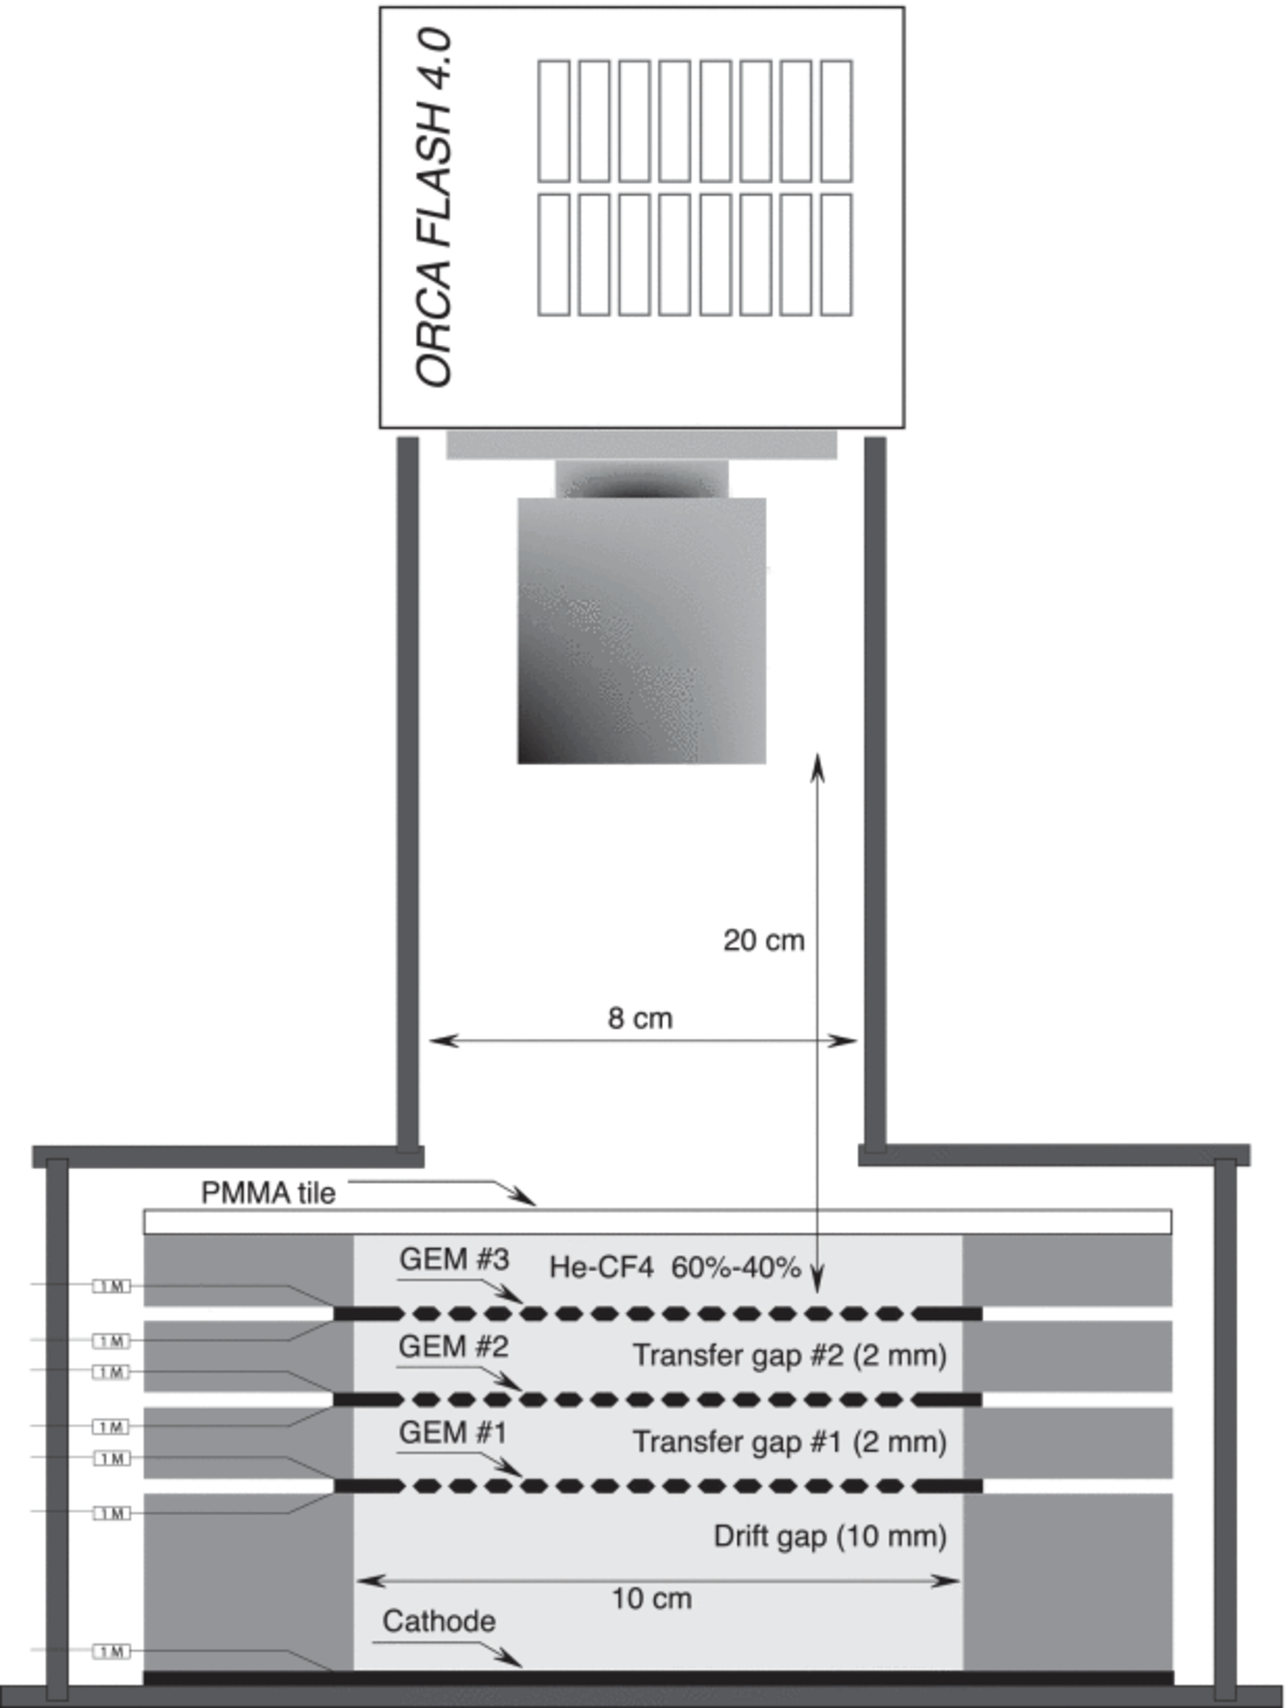
\includegraphics[width=0.65\textwidth]{image_files/orange1.pdf}
\caption{Configuração experimental do protótipo LEMOn: (A) gaiola de campo
elíptica com estrutura Triple-GEM; (B) fotomultiplicadora (PMT); (C) volume
escuro de distância adaptativa; (D) câmera sCMOS com lente.
Fonte:~\cite{bib:jinst_orange2}.}
\label{fig:lemon}
\end{figure}

\section{Conjuntos de Dados}
\label{sec:datasets}

\subsection{Dados de Simulação}

As imagens de simulação são produzidas com o software
Geant4~\cite{incerti2010geant4}, que modela a interação das partículas com o
gás do detector em nível microscópico. Para cada evento simulado, os elétrons
de ionização são propagados pelo campo de deriva e amplificados pelo
Triple-GEM, gerando uma imagem bidimensional de $2048 \times 2048$ pixels.

Para a dissertação de mestrado, foram utilizados dados para energias de 1, 3,
6, 10, 30 e 60~keV para recuos eletrônicos (ER) e nucleares (NR), com 100
imagens por combinação energia-tipo. A Figura~\ref{fig:track_generator} mostra
um exemplo de imagem simulada para um recuo eletrônico de 60~keV, juntamente
com sua máscara de \textit{ground truth}.

\begin{figure}[H]
\centering
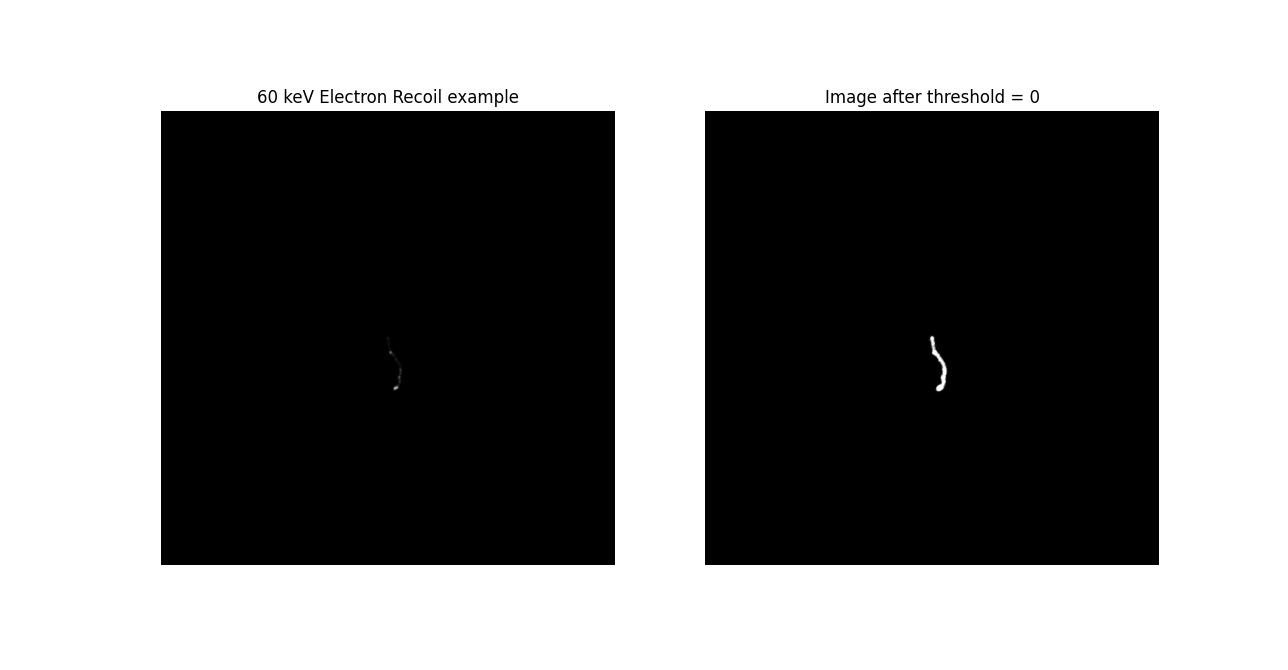
\includegraphics[width=\textwidth]{image_files/track_generator.png}
\caption{Exemplo de imagem de simulação Geant4 para um recuo eletrônico de
60~keV (esquerda) e sua máscara de \textit{ground truth} com threshold zero
(direita), indicando os pixels efetivamente ativados pela partícula.}
\label{fig:track_generator}
\end{figure}

Para o presente trabalho de doutorado, foram acrescentados dados de simulação
cobrindo a faixa de \textbf{0,25 a 1~keV} — exatamente a região de maior
interesse físico para WIMPs leves — combinados com ruído eletrônico real
proveniente dos \textit{runs} recentes 12163, 12166, 12168 e 12175 do
experimento.

Uma característica fundamental dos dados é o extremo desbalanceamento de
classes: em média, apenas \textbf{0,11\%} dos pixels de cada imagem contêm
sinal de evento. Os outros $99{,}89\%$ registram apenas ruído eletrônico. Esse
desbalanceamento torna as métricas clássicas como acurácia inadequadas para
avaliar o desempenho dos algoritmos.

\subsection{Dados Reais de Ruído}

Para reproduzir fielmente as condições do detector, imagens de ruído real foram
adquiridas reduzindo a tensão $V_{\text{GEM}}$ até eliminar a multiplicação de
avalanche — registrando assim apenas o ruído eletrônico da câmera. A
distribuição de intensidade de cada pixel foi caracterizada individualmente a
partir de 6.478 imagens de ruído, permitindo a construção de um simulador
Monte Carlo de ruído realista. A Figura~\ref{fig:noise_insertion} ilustra o
efeito da inserção de ruído sobre uma imagem de simulação.

\begin{figure}[H]
\centering
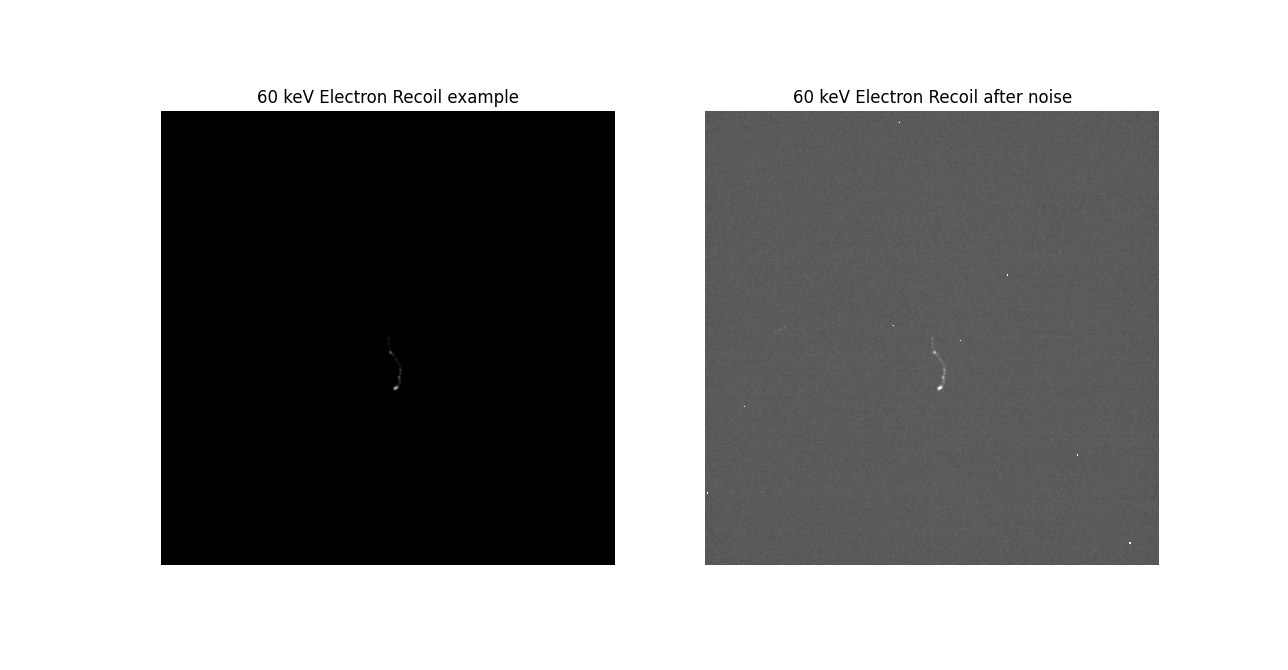
\includegraphics[width=\textwidth]{image_files/noise_insertion.png}
\caption{Efeito da inserção de ruído eletrônico sobre uma imagem de simulação.
À esquerda: imagem de simulação pura. À direita: imagem após inserção do ruído
real do detector, representando as condições reais de aquisição.}
\label{fig:noise_insertion}
\end{figure}


%%==========================================================
\chapter{Revisão: Algoritmo de Reconstrução e Seleção de Pixels}
\label{chap:reco}
%%==========================================================

\section{Visão Geral do Pipeline de Reconstrução}
\label{sec:pipeline}

O pipeline de reconstrução do Experimento CYGNO transforma uma imagem bruta da
câmera sCMOS em grandezas físicas mensuráveis — posição, energia e direção das
partículas interagentes. O processo é dividido em três grandes etapas:
\textbf{(1) Pré-processamento}, que seleciona os pixels de sinal;
\textbf{(2) Agrupamento} (\textit{Clustering}), que agrupa pixels de sinal em
clusters representando eventos individuais; e \textbf{(3) Extração de
características}, que computa as grandezas físicas de interesse para cada
cluster.

A Figura~\ref{fig:reco_flow} ilustra o fluxograma original do algoritmo de
reconstrução, mostrando a sequência de etapas que transformam a imagem bruta
em informação física.

\begin{figure}[H]
\centering
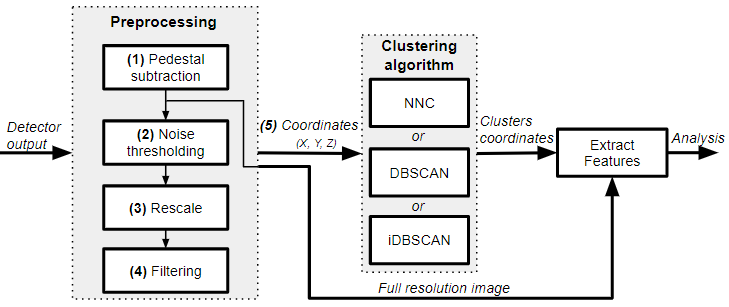
\includegraphics[width=0.75\textwidth]{image_files/fluxgram_algorithm.PNG}
\caption{Fluxograma do algoritmo de reconstrução do Experimento CYGNO. A
imagem bruta passa pelas etapas de pré-processamento (subtração de pedestal,
limiarização, rebinning, filtragem) antes do agrupamento iDBSCAN e extração de
características. Adaptado de~\cite{baracchini2020density}.}
\label{fig:reco_flow}
\end{figure}

\section{Pré-processamento}
\label{sec:preprocessing}

O pré-processamento é composto por quatro etapas sequenciais, cuja finalidade
coletiva é reduzir o volume de pixels enviados ao agrupamento, retendo apenas
os pixels com probabilidade razoável de serem sinal.

\subsection{Subtração de Pedestal}

A imagem bruta da câmera pode ser descrita como a soma da contribuição real da
partícula e do ruído eletrônico:
\begin{equation}
    I_{\text{real}}[x, y] = I_{\text{truth}}[x, y] + \eta[x, y]
    \label{eq:noise_model}
\end{equation}
onde $I_{\text{real}}[x,y]$ é a imagem adquirida, $I_{\text{truth}}[x,y]$ é
a imagem ideal (sem ruído) e $\eta[x,y]$ é o ruído eletrônico, com média
não-nula e distribuição independente por pixel.

A subtração de pedestal remove a média do ruído de cada pixel utilizando um
mapa de pedestal (\textit{pedmap}), obtido a partir de imagens adquiridas com
a câmera obstruída:
\begin{equation}
    I_{\text{ped}}[x, y] = I_{\text{real}}[x, y] - \bar{\eta}[x, y]
    \label{eq:pedestal}
\end{equation}

Após essa etapa, a maioria dos pixels de fundo apresenta valores próximos de
zero, enquanto os pixels de sinal mantêm intensidade positiva. A
Figura~\ref{fig:pedestal_subtraction} ilustra o efeito da subtração de
pedestal sobre os histogramas de intensidade.

\begin{figure}[H]
     \centering
     \begin{subfigure}[b]{0.47\textwidth}
         \centering
         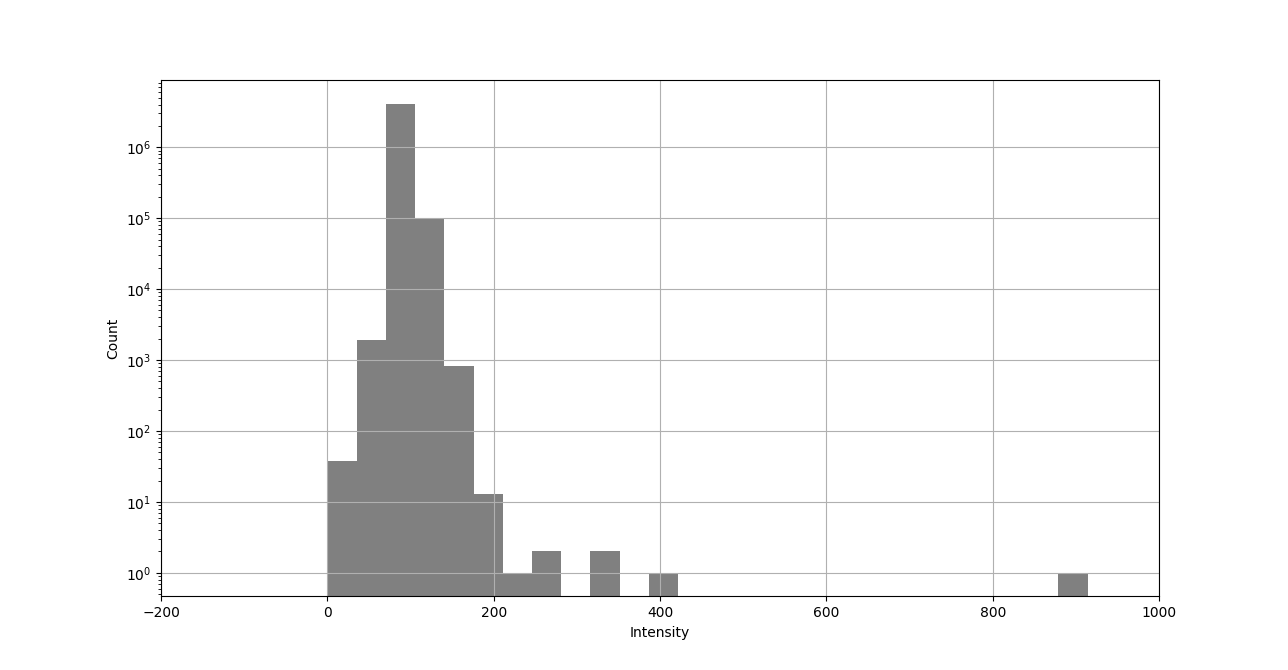
\includegraphics[width=\textwidth]{image_files/noise_before_ped.png}
         \caption{Histograma antes da subtração de pedestal.}
         \label{fig:hist_before_ped}
     \end{subfigure}
     \hfill
     \begin{subfigure}[b]{0.47\textwidth}
         \centering
         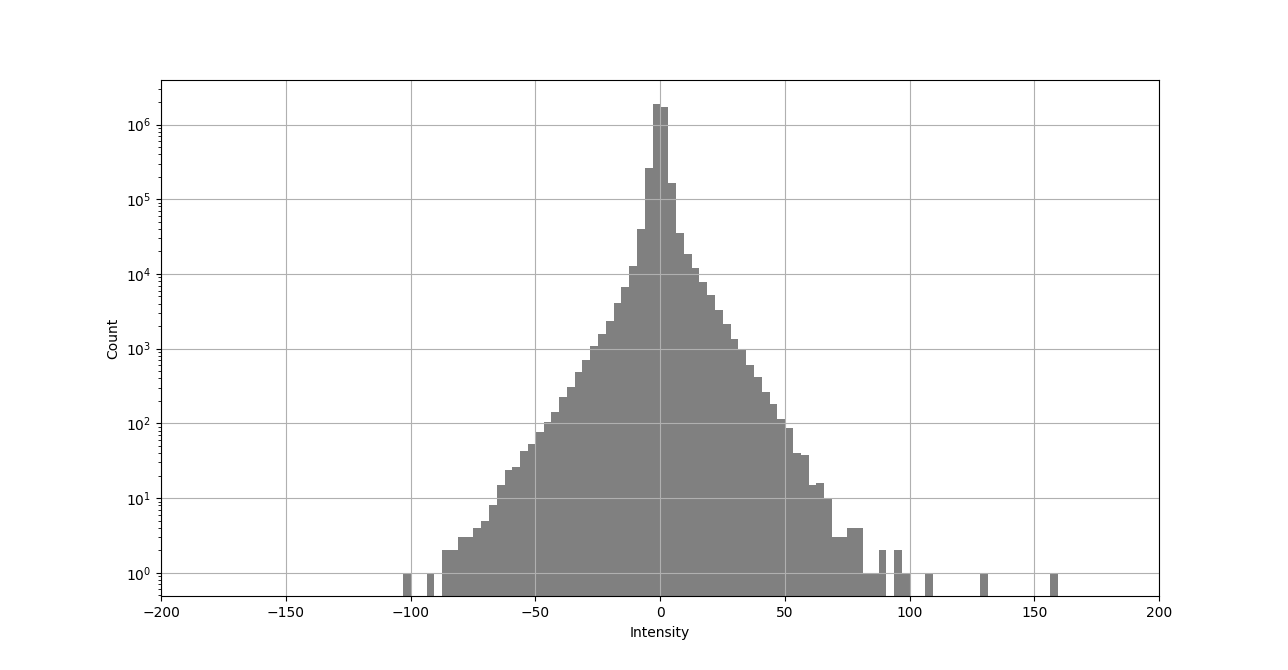
\includegraphics[width=\textwidth]{image_files/noise_after_ped.png}
         \caption{Histograma após a subtração de pedestal.}
         \label{fig:hist_after_ped}
     \end{subfigure}
     \caption{Efeito da subtração de pedestal sobre o histograma de intensidade
     de uma imagem. Após a subtração, a maioria dos pixels de fundo apresenta
     valores próximos de zero, facilitando a etapa de limiarização subsequente.}
     \label{fig:pedestal_subtraction}
\end{figure}

\subsection{Limiarização}

Após a subtração do pedestal, um limiar baseado no desvio padrão do ruído de
cada pixel é aplicado:
\begin{equation}
    I_{\text{thresh}}[x, y] = \begin{cases}
        I_{\text{ped}}[x, y] & \text{se } I_{\text{ped}}[x, y] > n \cdot \sigma[x, y] \\
        0 & \text{caso contrário}
    \end{cases}
    \label{eq:threshold}
\end{equation}
onde $\sigma[x,y]$ é o desvio padrão do ruído do pixel $(x,y)$ e $n \approx
1{,}3$ é o fator de limiarização adotado pelo experimento. Este passo reduz
drasticamente o número de pixels não-nulos, mas pode eliminar pixels de sinal
de baixa intensidade, comprometendo a detecção de eventos de baixa energia.

\subsection{Rebinning}

O \textit{rebinning} agrupa blocos de $4 \times 4$ pixels em um único pixel,
reduzindo a resolução de $2048 \times 2048$ para $512 \times 512$. O objetivo
é diminuir o número de pontos enviados ao algoritmo de agrupamento, reduzindo
o custo computacional. Contudo, essa operação implica perda de resolução
espacial, que pode ser crítica para eventos de baixa energia cujos traços
ocupam apenas poucos pixels.

\subsection{Filtragem e Redução de Ruído}

Na versão original do algoritmo, após o \textit{rebinning} é aplicado um
filtro de mediana com janela $4 \times 4$ (15 vizinhos), seguido de um
algoritmo redutor de ruído que elimina pixels isolados esparsos. Essa última
etapa é computacionalmente custosa — responsável por grande parte do tempo
total de processamento — e representa uma das principais motivações para a
substituição por abordagens baseadas em aprendizado profundo.

\section{Agrupamento: iDBSCAN}
\label{sec:idbscan}

Após o pré-processamento, os pixels sobreviventes (coordenadas e intensidades)
são enviados ao algoritmo iDBSCAN (\textit{Intensity-based
DBSCAN})~\cite{baracchini2020density}. O iDBSCAN é uma extensão do
DBSCAN~\cite{dbscan1996} que incorpora a intensidade dos pixels como peso na
definição de densidade local, resultando em melhor desempenho na identificação
de clusters de partículas em comparação com o DBSCAN convencional e o NNC
(\textit{Nearest Neighbor Clustering}).

Os parâmetros fundamentais do iDBSCAN são:
\begin{itemize}
    \item \texttt{eps}: raio de busca de vizinhança;
    \item \texttt{min\_samples}: número mínimo de pixels para formar um
    cluster;
    \item \texttt{dir\_radius}: raio para cálculo de direcionalidade.
\end{itemize}

O número de pontos enviados ao iDBSCAN impacta diretamente seu tempo de
execução. A relação entre número de pixels de entrada e tempo de agrupamento
é supralinear — comportamento que motiva fortemente a redução do número de
pixels pela etapa de pré-processamento. A Figura~\ref{fig:dbscan_time} ilustra
essa relação, evidenciando o benefício de enviar menos pixels ao algoritmo de
agrupamento.

\begin{figure}[H]
\centering
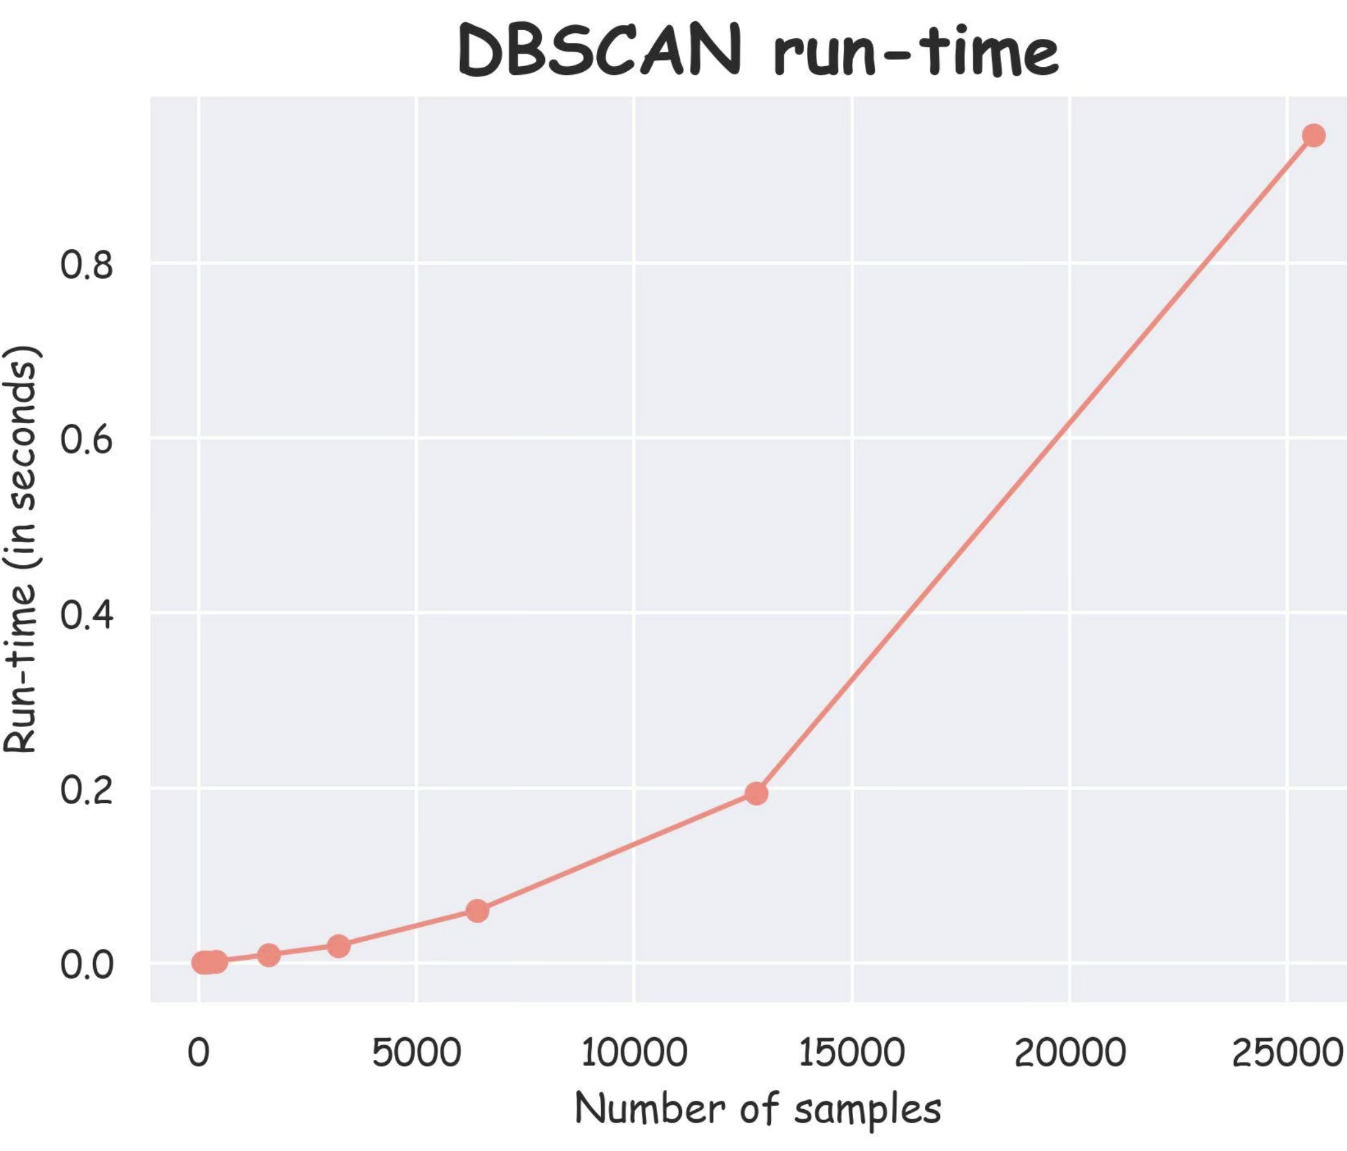
\includegraphics[width=0.70\textwidth]{quali_images/dbscan_runtime.png}
\caption{Tempo de execução do iDBSCAN em função do número de pixels de
entrada. A relação supralinear evidencia a importância de reduzir o número de
pixels na etapa de pré-processamento. Fonte: apresentação à colaboração CYGNO
(2024).}
\label{fig:dbscan_time}
\end{figure}

\section{Extração de Características}
\label{sec:features}

Para cada cluster identificado pelo iDBSCAN, um conjunto de características é
calculado, incluindo:
\begin{itemize}
    \item \textbf{Integral do cluster} ($S_c$): soma das intensidades dos
    pixels do cluster, proporcional à energia depositada pela partícula;
    \item \textbf{Posição}: centroide e distribuição espacial do cluster;
    \item \textbf{Formato}: elipticidade, eixos principais, comprimento;
    \item \textbf{Direcionalidade}: ângulo do eixo principal do cluster em
    relação ao plano de detecção.
\end{itemize}

A grandeza física mais relevante para este trabalho é a integral do cluster
$S_c$, que é convertida em energia pela relação:
\begin{equation}
    E\,[\text{keV}] = k \cdot S_c
    \label{eq:energy}
\end{equation}
onde $k$ é uma constante de calibração determinada a partir de fontes
radioativas de referência (tipicamente $^{55}$Fe, que emite a 5,9~keV).

\section{O Gargalo: Seleção de Pixels em Baixas Energias}
\label{sec:bottleneck}

A etapa de seleção de pixels no pré-processamento é o gargalo do pipeline por
dois motivos interligados:

\textbf{1.\ Desempenho físico:} Para eventos de baixa energia (abaixo de
6~keV), o sinal dos pixels de evento é comparável ao ruído eletrônico. A
limiarização baseada em $n \cdot \sigma$ elimina uma fração significativa dos
pixels de sinal verdadeiro (\textit{falsos negativos}), comprometendo a
estimativa de energia. Ao mesmo tempo, pixels de ruído com intensidade acima
do limiar são incorretamente incluídos (\textit{falsos positivos}), gerando
clusters espúrios.

\textbf{2.\ Desempenho computacional:} O algoritmo original envia
${\sim}50{.}000$ pixels ao iDBSCAN por imagem, consumindo tempo de
processamento significativo. Uma seleção de pixels mais precisa reduziria
drasticamente esse número, acelerando todo o pipeline.

A Figura~\ref{fig:pipeline_motivation} apresenta o pipeline de reconstrução
com destaque à etapa de pré-processamento, mostrando onde o presente trabalho
concentra suas contribuições.

\begin{figure}[H]
\centering

\includegraphics[width=\textwidth]{quali_images/cygno_preprocessing_flow.png}
\caption{Pipeline de reconstrução do Experimento CYGNO com destaque à etapa
de pré-processamento. O trabalho proposto atua na substituição das etapas de
filtragem e redução de ruído por uma rede neural U-Net, melhorando tanto o
desempenho físico quanto o computacional. Fonte: apresentação à colaboração
CYGNO (2024).}
\label{fig:pipeline_motivation}
\end{figure}


%%==========================================================
\chapter{Trabalho Anterior: Comparação de Filtros na Dissertação de Mestrado}
\label{chap:dissertation}
%%==========================================================

Este capítulo resume os resultados da dissertação de mestrado do
autor~\cite{lopes2019study}, estabelecendo a ponte narrativa entre o trabalho
realizado e as questões que motivam o presente doutorado.

\section{Metodologia e Filtros Avaliados}
\label{sec:dissertation_context}

A dissertação propôs uma metodologia de avaliação baseada em dados de simulação
(Geant4, energias de 1 a 60~keV, ER e NR) combinados com ruído real do
detector, utilizando o F1-score como métrica principal — adequada ao extremo
desbalanceamento de classes (${\sim}0{,}1\%$ de sinal). Foram comparados
filtros de média ($W=17$), gaussiano ($W=17$), mediana ($W=15$), a rede neural
U-Net~\cite{ronneberger2015u} e o algoritmo original do CYGNO (limiarização
por $n \cdot \sigma_{\text{ruído}}$). A Figura~\ref{fig:simulation_env}
apresenta o diagrama do ambiente de avaliação.

\begin{figure}[H]
\centering
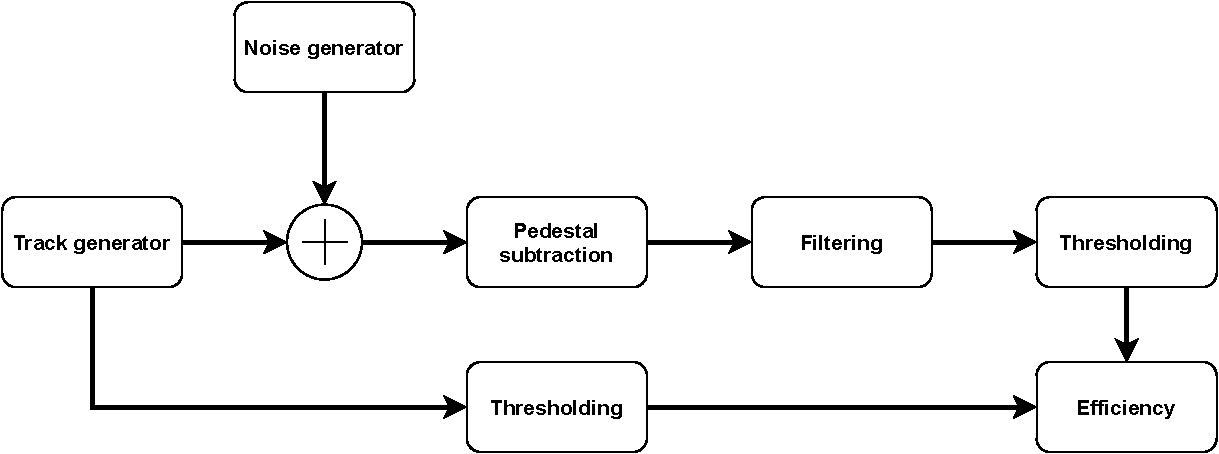
\includegraphics[width=\textwidth]{image_files/diagrama_dissertacao.pdf}
\caption{Diagrama do ambiente de avaliação proposto na dissertação de
mestrado. Imagens de simulação e ruído real são combinadas, processadas por
cada filtro/algoritmo e avaliadas pela métrica F1-score.}
\label{fig:simulation_env}
\end{figure}

\section{Resultados Principais}
\label{sec:dissertation_results}

A Tabela~\ref{tab:f1_results} sintetiza o desempenho de seleção de pixels.
A U-Net alcançou o melhor F1-score (0,873), com a menor variância entre
algoritmos, superando o filtro de mediana (0,820) e, especialmente, o
algoritmo original (0,137). Esse resultado evidencia que a limiarização
simples por $n \cdot \sigma$ é inadequada para a seleção de pixels em baixa
razão sinal-ruído.

\begin{table}[H]
\centering
\caption{Resumo dos resultados de F1-score na seleção de pixels (média $\pm$
desvio padrão sobre todos os eventos e energias do conjunto de teste).}
\label{tab:f1_results}
\begin{tabular}{lcc}
\toprule
\textbf{Algoritmo} & \textbf{Parâmetro} & \textbf{F1-score ($\mu \pm \sigma$)} \\
\midrule
U-Net              & (treinado)  & $\mathbf{0{,}873 \pm 0{,}060}$ \\
Mediana            & $W = 15$    & $0{,}820 \pm 0{,}127$           \\
Média              & $W = 17$    & $0{,}800 \pm 0{,}184$           \\
Gaussiano          & $W = 17$    & $0{,}771 \pm 0{,}225$           \\
CYGNO original     & ---         & $0{,}137 \pm 0{,}127$           \\
\bottomrule
\end{tabular}
\fonte{Lopes (2022).}
\end{table}

Na reconstrução de energia em simulação, a U-Net e o filtro de mediana
apresentaram $R^2$ mais próximo de 1 para todas as energias, enquanto o
algoritmo original obteve os piores valores. Em dados reais ($^{55}$Fe,
5,9~keV), o filtro de mediana reproduziu a distribuição de energia do
algoritmo original com fidelidade estatística (Kolmogorov-Smirnov:
$p = 0{,}514$), com tempo de processamento \textbf{4,3 vezes menor}
(67,6~s vs.\ 293,8~s por imagem). A redução é atribuída à eliminação do
algoritmo redutor de ruído e à diminuição de duas ordens de magnitude no
número de pixels enviados ao iDBSCAN.

\section{A Pergunta em Aberto}
\label{sec:dissertation_conclusion}

Os resultados da dissertação demonstraram que a U-Net é a melhor abordagem
para seleção de pixels no CYGNO. Contudo, os dados utilizados cobriam apenas
energias \textbf{acima de 1~keV} — regime onde o sinal ainda é
suficientemente distinguível do ruído. A questão fundamental que motiva o
presente doutorado é: \textbf{qual é o desempenho da U-Net para eventos de
energias muito baixas, na faixa de 0,25 a 1~keV?} Essa faixa corresponde ao
regime de máximo interesse físico para WIMPs leves e apresenta a maior
dificuldade de seleção de pixels — o sinal é praticamente indistinguível do
ruído eletrônico por métodos clássicos.


%%==========================================================
\chapter{Metodologia: U-Net para Baixas Energias}
\label{chap:methodology}
%%==========================================================

\section{Visão Geral e Mudanças em Relação ao Trabalho Anterior}
\label{sec:changes}

O presente trabalho estende a investigação iniciada na dissertação de mestrado
com três mudanças fundamentais:
\begin{enumerate}
    \item \textbf{Novos dados de simulação em baixas energias}: energias de
    0,25; 0,5 e 1~keV para ER e NR, combinados com ruído real de
    \textit{runs} mais recentes do experimento (12163, 12166, 12168 e 12175);
    \item \textbf{Nova função de perda — Focal Loss}: substituição da
    entropia cruzada binária pela Focal Loss~\cite{lin2017focal} com
    $\alpha = 4$, para priorizar a revocação no regime de extremo
    desbalanceamento;
    \item \textbf{Avaliação \textit{end-to-end} no pipeline de reconstrução}:
    a U-Net treinada é integrada ao pipeline completo, com métricas de
    detecção de eventos, tempo de processamento e estimativa de energia.
\end{enumerate}

Todas essas mudanças são motivadas pelo objetivo de verificar o desempenho da
U-Net na faixa de energia de máximo interesse físico para a detecção de
matéria escura leve.

\section{Seleção de Pixels como Segmentação Semântica}
\label{sec:semantic_seg}

A tarefa de seleção de pixels pode ser formulada como um problema de
\textbf{segmentação semântica binária}: dado uma imagem de
$2048 \times 2048$ pixels, classificar cada pixel individualmente como
\textit{sinal} (contém contribuição de um evento de partícula) ou
\textit{fundo} (contém apenas ruído eletrônico). Diferentemente de uma
classificação global da imagem, a segmentação semântica preserva a resolução
espacial completa, permitindo a localização precisa dos pixels de evento.

Essa formulação apresenta três desafios principais no contexto do CYGNO:
\begin{itemize}
    \item \textbf{Extremo desbalanceamento de classes}: apenas ${\sim}0{,}1\%$
    dos pixels são sinal — uma razão de ${\sim}1{:}1000$ entre classes;
    \item \textbf{Baixa razão sinal-ruído}: para energias abaixo de 1~keV,
    os pixels de sinal possuem intensidades comparáveis ao ruído eletrônico;
    \item \textbf{Variabilidade morfológica}: os traços de recuos eletrônicos
    (ER) e nucleares (NR) apresentam morfologias distintas — ER produzem
    traços mais longos e curvos, enquanto NR geram deposições mais compactas
    e pontuais. Abaixo de 10~keV, as distribuições de intensidade de ambos
    os tipos tornam-se muito similares, dificultando a segmentação.
\end{itemize}

A abordagem baseada em visão computacional clássica (filtros espaciais
seguidos de limiarização) requer a definição manual de parâmetros que
dependem da energia e do tipo de partícula. A U-Net, por outro lado, aprende
esses padrões diretamente dos dados de treinamento, substituindo a engenharia
manual de características por um processo de otimização.

\section{Geração de Dados de Treinamento}
\label{sec:data_generation}

O processo de geração de dados de treinamento é um aspecto crítico da
metodologia. O pipeline completo é ilustrado na
Figura~\ref{fig:training_flow} e consiste nos seguintes passos:

\begin{enumerate}
    \item \textbf{Seleção de imagens de simulação}: imagens Geant4 para
    energias de 0,25 a 60~keV (ER e NR) são selecionadas aleatoriamente do
    conjunto de simulação;
    \item \textbf{Aumento de dados}: transformações de rotação (ângulo
    $\theta$ aleatório) e translação ($x_0, y_0$) são aplicadas \emph{antes}
    da inserção do ruído, seguindo a equação:
\end{enumerate}

\begin{equation}
    \begin{bmatrix} x' \\ y' \\ 1 \end{bmatrix}
    =
    \begin{bmatrix}
        \cos\theta & -\sin\theta & x_0 \\
        \sin\theta &  \cos\theta & y_0 \\
        0          &  0          & 1
    \end{bmatrix}
    \begin{bmatrix} x \\ y \\ 1 \end{bmatrix}
    \label{eq:augmentation}
\end{equation}

\begin{enumerate}
    \setcounter{enumi}{2}
    \item \textbf{Definição do \textit{ground truth}}: a máscara binária é
    obtida com \textit{threshold} zero na imagem de simulação pura:
    $I_{\text{truth}}[x,y] > 0 \Rightarrow$ sinal (1); caso contrário,
    fundo (0);
    \item \textbf{Inserção de ruído real}: uma imagem de ruído é selecionada
    aleatoriamente dentre os \textit{runs} disponíveis (12163, 12166, 12168,
    12175) e adicionada à imagem simulada, preservando as características
    reais do detector;
    \item \textbf{Subtração de pedestal}: o mapa de pedestal é subtraído,
    reproduzindo a primeira etapa do pipeline de reconstrução.
\end{enumerate}

A aplicação das transformações de aumento \emph{antes} da inserção do ruído é
uma decisão de projeto importante: se as transformações fossem aplicadas após
a adição de ruído, os padrões de ruído seriam rotacionados junto com o evento,
criando artefatos que não correspondem à realidade do detector. Da mesma
forma, o ruído é selecionado aleatoriamente dentre os \textit{runs}
disponíveis para expor a rede a diferentes condições operacionais.

\begin{figure}[H]
\centering

\includegraphics[width=\textwidth]{quali_images/cygno_preprocessing_flow.png}
\caption{Pipeline de geração de dados de treinamento da U-Net. Imagens de
simulação (0,25--60~keV, ER e NR) são combinadas com ruído real de
\textit{runs} recentes (12163, 12166, 12168 e 12175) após aumento de dados
por rotação e translação. O \textit{threshold} zero na simulação pura define
a máscara de \textit{ground truth}. Fonte: apresentação à colaboração CYGNO
(2024).}
\label{fig:training_flow}
\end{figure}

O conjunto de dados resultante é dividido em:
\begin{itemize}
    \item \textbf{2.000 imagens de treino}: abrangendo todas as energias e
    tipos de partícula, com ruído real de diferentes \textit{runs};
    \item \textbf{500 imagens de validação}: monitoramento do
    \textit{overfitting} durante o treinamento;
    \item \textbf{500 imagens de teste}: avaliação final, com imagens nunca
    vistas durante o treinamento.
\end{itemize}

Para a avaliação no pipeline de reconstrução, as imagens de teste são
restringidas à faixa de \textbf{0,25 a 1~keV}, com exatamente \textbf{1
evento} (NR ou ER) por imagem — permitindo uma avaliação precisa da taxa de
detecção e da estimativa de energia.

\section{Arquitetura da U-Net}
\label{sec:unet_architecture}

A U-Net~\cite{ronneberger2015u}, originalmente proposta para segmentação de
imagens biomédicas, é uma rede totalmente convolucional (FCN) com arquitetura
encoder-decoder e conexões de salto (\textit{skip connections}). Sua
aplicação ao CYGNO é particularmente adequada por duas razões: (1) funciona
bem com conjuntos de dados de tamanho moderado, e (2) preserva a informação
espacial de alta resolução necessária para a localização precisa dos pixels
de evento.

A arquitetura foi adaptada para acomodar imagens de $2048 \times 2048$ pixels
e possui a seguinte estrutura:
\begin{itemize}
    \item \textbf{Encoder (contração)}: 5 estágios de dupla convolução com
    \textit{batch normalization} e ativação ReLU, seguidos de
    max-pooling $2 \times 2$. Os mapas de características crescem em
    profundidade: 16 $\to$ 32 $\to$ 48 $\to$ 64 $\to$ 128 filtros, enquanto
    a resolução espacial é reduzida progressivamente de $2048^2$ até
    $64^2$;
    \item \textbf{Bottleneck}: duas camadas convolucionais com 128 filtros na
    resolução mínima ($64 \times 64$), onde são capturadas as representações
    mais abstratas;
    \item \textbf{Decoder (expansão)}: 5 estágios de \textit{upsampling}
    $2 \times 2$ com concatenação das ativações correspondentes do encoder
    (\textit{skip connections}), seguidos de dupla convolução. Os mapas de
    características diminuem: 128 $\to$ 64 $\to$ 48 $\to$ 32 $\to$ 16;
    \item \textbf{Camada de saída}: convolução $1 \times 1$ com ativação
    Sigmoide, produzindo um mapa de probabilidade pixel a pixel
    $p \in [0, 1]$.
\end{itemize}

As \textit{skip connections} são fundamentais para este problema: ao
concatenar os mapas de alta resolução do encoder com os mapas reconstruídos do
decoder, a rede preserva detalhes finos do sinal mesmo após o gargalo
(\textit{bottleneck}). Sem essas conexões, a informação de posição dos
pixels de sinal — que ocupam apenas ${\sim}0{,}1\%$ da imagem — seria
perdida na compressão.

A saída da U-Net é um mapa de probabilidades da mesma resolução da entrada
($2048 \times 2048$). Um limiar $t$ é aplicado para obter a máscara binária:
\begin{equation}
    M[x, y] = \begin{cases}
        1 & \text{se } p_{\text{U-Net}}[x, y] > t \\
        0 & \text{caso contrário}
    \end{cases}
    \label{eq:binary_mask}
\end{equation}

A arquitetura completa é apresentada no Apêndice~\ref{apend:unet}.

\section{Focal Loss: Tratando o Desbalanceamento Extremo de Classes}
\label{sec:focal_loss}

O extremo desbalanceamento de classes é o maior desafio do treinamento. Com
apenas ${\sim}0{,}1\%$ de pixels de sinal, a entropia cruzada binária padrão
é dominada pela classe majoritária (fundo) — a rede pode atingir
$> 99{,}9\%$ de acurácia simplesmente classificando todos os pixels como
fundo, sem aprender os padrões de sinal.

A \textbf{Focal Loss}~\cite{lin2017focal}, proposta originalmente para
detecção de objetos densos, generaliza a entropia cruzada binária adicionando
dois mecanismos de controle:

\begin{equation}
    FL(p_t) = -\alpha_t \cdot (1 - p_t)^{\gamma} \cdot \log(p_t)
    \label{eq:focal_loss}
\end{equation}

onde:
\begin{itemize}
    \item $p_t$ é a probabilidade prevista para a classe correta;
    \item $\gamma \geq 0$ é o \textbf{parâmetro de foco}: reduz a
    contribuição de exemplos fáceis (bem classificados). Para $\gamma = 0$,
    recupera-se a entropia cruzada padrão. Valores maiores concentram o
    treinamento em exemplos difíceis. Valor utilizado: $\gamma = 2$;
    \item $\alpha_t$ é o \textbf{fator de balanceamento de classes}. Para a
    classe de sinal: $\alpha_t = \alpha$; para o fundo:
    $\alpha_t = 1 - \alpha$.
\end{itemize}

O parâmetro $\alpha = 4$ foi selecionado para \textbf{priorizar a Revocação
em detrimento da Precisão}. A justificativa é física: no contexto do
experimento, perder um evento verdadeiro (falso negativo) é mais custoso do
que incluir alguns pixels de fundo adicionais (falsos positivos). Os pixels
de fundo extras geram clusters falsos que podem ser identificados e
descartados na análise posterior. Contudo, pixels de evento perdidos resultam
em subestimação irreversível da energia — particularmente grave na faixa de
0,25 a 1~keV, onde cada pixel de sinal contém informação preciosa.

Para efeito de comparação, a entropia cruzada binária padrão é:
\begin{equation}
    \text{BCE}(p_t) = -\log(p_t)
    \label{eq:bce}
\end{equation}

A Focal Loss adiciona o fator $(1 - p_t)^\gamma$, que suprime a contribuição
de pixels facilmente classificados (ruído de fundo com $p_t \approx 0$).
Com $\gamma = 2$, um pixel classificado corretamente com $p_t = 0{,}9$ tem
sua contribuição à perda reduzida por um fator de 100 em relação a $\gamma =
0$. Isso força a rede a se concentrar nos pixels ambíguos — exatamente os
pixels de sinal de baixa energia, que são os exemplos mais difíceis.

\section{Configuração de Treinamento}
\label{sec:training_config}

Os parâmetros de treinamento utilizados são:
\begin{itemize}
    \item \textbf{Otimizador}: Adam~\cite{defossez2020convergence}, taxa de
    aprendizado $= 0{,}02$;
    \item \textbf{Épocas}: 50, com 450 passos por época;
    \item \textbf{Regularização}: \textit{Batch Normalization} em cada bloco
    convolucional, para estabilizar o treinamento e permitir taxas de
    aprendizado mais altas;
    \item \textbf{Função de perda}: Focal Loss com $\alpha = 4$ e
    $\gamma = 2$;
    \item \textbf{Critério de parada}: monitoramento da Focal Loss de
    validação ao longo das épocas, sem indicação de \textit{overfitting}
    após 50 épocas.
\end{itemize}

\section{Métricas de Avaliação}
\label{sec:metrics}

Dada a inadequação de métricas como acurácia e ROC para problemas de classes
altamente desbalanceadas, o desempenho é avaliado por:

\begin{equation}
    \text{Precisão} = \frac{VP}{VP + FP}
    \label{eq:precision}
\end{equation}
\begin{equation}
    \text{Revocação} = \frac{VP}{VP + FN}
    \label{eq:recall}
\end{equation}

onde $VP$ são os pixels de sinal corretamente classificados, $FP$ são pixels
de fundo classificados como sinal e $FN$ são pixels de sinal classificados
como fundo. A Precisão indica a pureza da seleção; a Revocação indica a
completude da detecção.

Além das métricas de pixel, a avaliação \textit{end-to-end} no pipeline de
reconstrução utiliza:
\begin{itemize}
    \item \textbf{Taxa de detecção de eventos verdadeiros}: fração de imagens
    em que o evento real é detectado pelo iDBSCAN;
    \item \textbf{Número de clusters falsos}: clusters espúrios formados por
    pixels de ruído — indica a taxa de alarme falso;
    \item \textbf{Integral do cluster} ($S_c$): soma das intensidades dos
    pixels do cluster, proporcional à energia depositada. A comparação com o
    $S_c$ do \textit{ground truth} avalia a qualidade da estimativa de
    energia;
    \item \textbf{Tempo de processamento}: tempo total e por etapa,
    comparando os dois pipelines nas mesmas condições computacionais.
\end{itemize}

\section{Integração ao Pipeline de Reconstrução}
\label{sec:pipeline_integration}

A U-Net treinada é inserida no pipeline de reconstrução em substituição às
etapas de filtragem, rebinning e redução de ruído. A comparação entre o
pipeline original e o proposto é apresentada abaixo e ilustrada na
Figura~\ref{fig:pipeline_comparison}.

\medskip
\noindent\textbf{Pipeline original (Reco):}
\begin{enumerate}
    \item Subtração de pedestal
    \item Limiarização ($n \cdot \sigma$)
    \item Rebinning ($2048 \to 512$)
    \item Filtro de mediana ($4 \times 4$)
    \item Redução de ruído (pixels isolados)
    \item iDBSCAN $\to$ Extração de características
\end{enumerate}

\noindent\textbf{Pipeline proposto (Reco + U-Net):}
\begin{enumerate}
    \item Subtração de pedestal
    \item \textbf{U-Net} (segmentação semântica, $2048 \times 2048$)
    \item Limiarização do mapa de probabilidades
    \item iDBSCAN $\to$ Extração de características
\end{enumerate}

\begin{figure}[H]
\centering
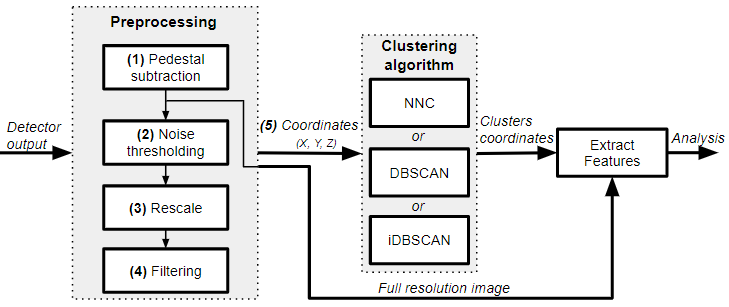
\includegraphics[width=0.75\textwidth]{image_files/fluxgram_algorithm.PNG}
\caption{Comparação esquemática dos pipelines. No pipeline proposto (Reco +
U-Net), a rede neural substitui as etapas de limiarização por $n\sigma$,
rebinning, filtragem e redução de ruído. Os parâmetros do iDBSCAN são mantidos
idênticos: \texttt{eps = 18}, \texttt{min\_samples = 20},
\texttt{dir\_radius = 35}, \texttt{nsigma = 0,2} (\texttt{branch =
winter23}).}
\label{fig:pipeline_comparison}
\end{figure}

O pipeline proposto apresenta duas vantagens estruturais:
\begin{enumerate}
    \item \textbf{Opera na resolução completa}: a U-Net processa imagens de
    $2048 \times 2048$ diretamente, sem a perda de resolução do rebinning
    para $512 \times 512$ — preservando informação espacial crucial para
    eventos de baixa energia cujos traços ocupam apenas poucos pixels;
    \item \textbf{Redução radical de pixels}: a U-Net entrega ao iDBSCAN
    apenas ${\sim}450$ pixels por imagem (somente os identificados como
    sinal), comparado a ${\sim}50{.}000$ no algoritmo original — uma redução
    de duas ordens de magnitude que impacta diretamente o tempo de
    agrupamento, cuja complexidade é supralinear com o número de pontos
    (cf.\ Figura~\ref{fig:dbscan_time}).
\end{enumerate}

Para a avaliação, cada imagem de teste contém exatamente 1 evento de NR ou ER
com energia de 0,25, 0,5 ou 1~keV. Todos os parâmetros do iDBSCAN são
mantidos idênticos nos dois pipelines para garantir que as diferenças
observadas sejam atribuídas exclusivamente à etapa de seleção de pixels.


%%==========================================================
\chapter{Resultados}
\label{chap:results}
%%==========================================================

Neste capítulo são apresentados os resultados obtidos com a integração da
U-Net ao pipeline de reconstrução do Experimento CYGNO, organizados em cinco
partes: (1) curvas de treinamento; (2) detecção de eventos e clusters falsos;
(3) tempo de processamento; (4) o resultado central — distribuições de
integral de cluster para cada energia; e (5) discussão dos resultados com
análise por energia e tipo de partícula.

\section{Treinamento da U-Net}
\label{sec:training_results}

A Figura~\ref{fig:training_curves} apresenta a evolução da Focal Loss ao
longo das 50 épocas de treinamento, para os conjuntos de treino e validação.

\begin{figure}[H]
\centering
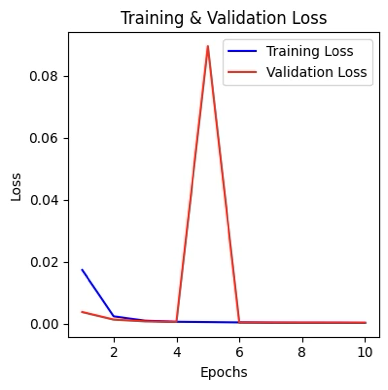
\includegraphics[width=\textwidth]{quali_images/loss_function_training_validation.png}
\caption{Evolução da Focal Loss durante o treinamento da U-Net. As curvas de
treino e validação convergem rapidamente (menos de 5 épocas) e permanecem
próximas ao longo de todas as 50 épocas, sem evidências de
\textit{overfitting}. Fonte: apresentação à colaboração CYGNO (2024).}
\label{fig:training_curves}
\end{figure}

As Figuras~\ref{fig:precision_curves} e~\ref{fig:recall_curves} detalham a
evolução das métricas de Precisão e Revocação.

\begin{figure}[H]
\centering
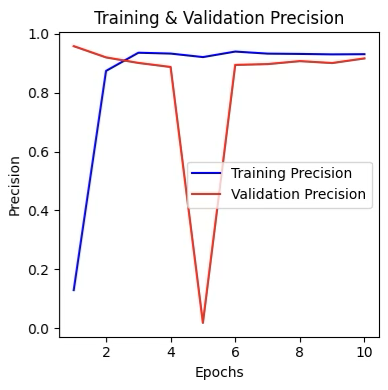
\includegraphics[width=0.72\textwidth]{quali_images/precision.png}
\caption{Precisão de treino e validação ao longo das épocas. O valor se
estabiliza em ${\sim}0{,}85$--$0{,}90$. A Precisão mede a fração dos pixels
selecionados pela U-Net que são efetivamente sinal — valores elevados indicam
baixa taxa de falsos positivos. Fonte: apresentação à colaboração CYGNO
(2024).}
\label{fig:precision_curves}
\end{figure}

\begin{figure}[H]
\centering
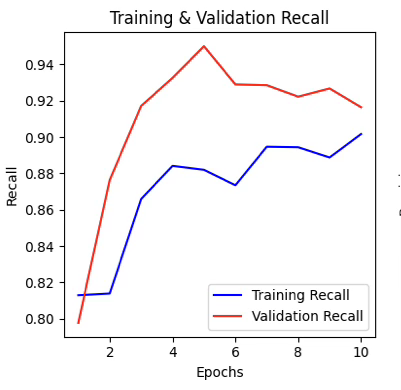
\includegraphics[width=0.72\textwidth]{quali_images/recall.png}
\caption{Revocação de treino e validação ao longo das épocas. O valor supera
$0{,}88$, refletindo a priorização imposta pelo $\alpha = 4$ da Focal Loss. A
Revocação mede a fração dos pixels de sinal verdadeiros que foram corretamente
identificados — valores elevados indicam poucos eventos perdidos. Fonte:
apresentação à colaboração CYGNO (2024).}
\label{fig:recall_curves}
\end{figure}

Os resultados de treinamento evidenciam três características:
\begin{itemize}
    \item \textbf{Convergência rápida}: a Focal Loss atinge valores estáveis
    em menos de 5 épocas, indicando que a rede aprende rapidamente os padrões
    de sinal mesmo para baixas energias;
    \item \textbf{Ausência de \textit{overfitting}}: as curvas de treino e
    validação permanecem próximas ao longo de todas as 50 épocas, confirmando
    que a combinação de aumento de dados e \textit{batch normalization}
    previne a sobre-parametrização;
    \item \textbf{Revocação $>$ Precisão}: a Revocação ($> 0{,}88$) supera
    sistematicamente a Precisão ($0{,}85$--$0{,}90$), validando o efeito
    intencional do $\alpha = 4$ na Focal Loss. A rede prioriza a detecção
    completa de pixels de sinal, aceitando uma fração controlada de falsos
    positivos.
\end{itemize}

Esse comportamento é desejável: os falsos positivos geram clusters espúrios
que podem ser filtrados pelo iDBSCAN ou na análise posterior, enquanto falsos
negativos resultam em perda irreversível de informação de energia.

\section{Taxa de Detecção e Eventos Falsos}
\label{sec:fake_events}

Cada imagem de teste contém exatamente um evento (NR ou ER) em uma das três
energias avaliadas. A Figura~\ref{fig:fake_events} compara o número de
clusters falsos detectados pelo algoritmo original (Reco) e pelo pipeline
proposto (Reco + U-Net), discriminando por energia e tipo de partícula.

\begin{figure}[H]
\centering
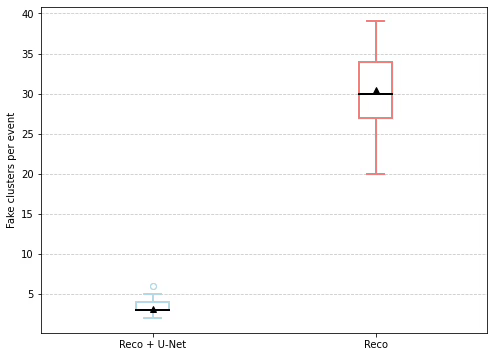
\includegraphics[width=\textwidth]{quali_images/fake_events.png}
\caption{Número de clusters falsos por evento: algoritmo original (Reco) vs.\
pipeline proposto (Reco + U-Net), para NR e ER a 0,25, 0,5 e 1~keV.
\textbf{99\% dos eventos verdadeiros foram detectados} pelo pipeline com
U-Net. A mediana de clusters falsos cai de ${\sim}30$ para ${\sim}3$--$4$,
uma redução de aproximadamente uma ordem de magnitude. Fonte: apresentação à
colaboração CYGNO (2024).}
\label{fig:fake_events}
\end{figure}

A análise detalhada revela:
\begin{itemize}
    \item \textbf{Taxa de detecção de 99\%}: a U-Net identifica corretamente
    a esmagadora maioria dos eventos verdadeiros em todas as energias e ambos
    os tipos de partícula. Os ${\sim}1\%$ de eventos não detectados
    correspondem a traços de energia extremamente baixa (0,25~keV) com poucos
    pixels ativados;
    \item \textbf{Redução de clusters falsos}: a mediana cai de ${\sim}30$
    (Reco) para ${\sim}3$--$4$ (Reco + U-Net). Essa redução é consequência
    direta da seletividade da U-Net: ao enviar apenas ${\sim}450$ pixels ao
    iDBSCAN (vs.\ ${\sim}50{.}000$), a probabilidade de formação de clusters
    espúrios a partir de pixels de ruído é drasticamente reduzida;
    \item \textbf{Consistência entre tipos de partícula}: o desempenho é
    similar para NR e ER, indicando que a U-Net aprendeu padrões genéricos de
    sinal vs.\ ruído, independentemente da morfologia do traço;
    \item \textbf{Impacto prático}: em um experimento de longa duração
    adquirindo milhões de imagens, reduzir os clusters falsos de ${\sim}30$
    para ${\sim}3$--$4$ por imagem diminui significativamente o volume de
    dados armazenados e o tempo de análise \textit{offline}.
\end{itemize}

\section{Tempo de Processamento}
\label{sec:processing_time}

A Figura~\ref{fig:processing_time} compara o tempo médio de processamento por
imagem entre os dois pipelines, detalhando a contribuição de cada etapa
(pré-processamento vs.\ agrupamento iDBSCAN).

\begin{figure}[H]
\centering
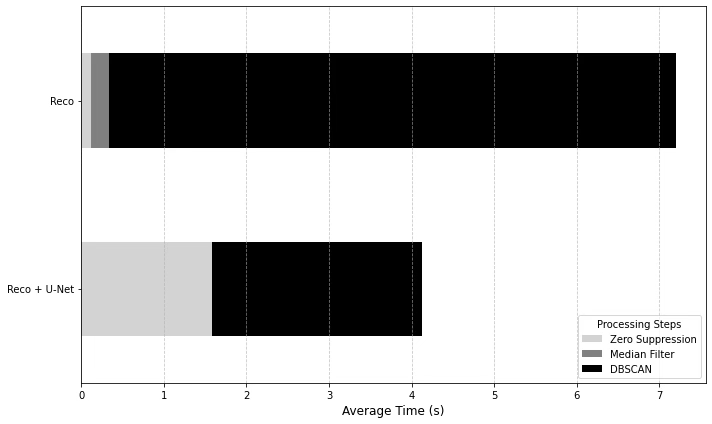
\includegraphics[width=\textwidth]{quali_images/processing_time.png}
\caption{Tempo de processamento por etapa: Reco (esquerda) vs.\ Reco + U-Net
(direita). A região cinza indica o pré-processamento; as demais barras indicam
o agrupamento iDBSCAN. Apesar de operar em imagens de resolução completa
($2048 \times 2048$), o pipeline com U-Net apresenta tempo total
significativamente menor. Fonte: apresentação à colaboração CYGNO (2024).}
\label{fig:processing_time}
\end{figure}

A redução de tempo é explicada por três fatores:
\begin{enumerate}
    \item \textbf{Eliminação do algoritmo redutor de ruído}: no pipeline
    original, esta é a etapa mais custosa — remove pixels isolados após a
    filtragem, iterando sobre os ${\sim}50{.}000$ pixels sobreviventes. No
    pipeline proposto, a U-Net já seleciona apenas os pixels relevantes,
    tornando essa etapa desnecessária;
    \item \textbf{Redução de pixels para o iDBSCAN}: o pipeline com U-Net
    envia apenas ${\sim}450$ pixels ao iDBSCAN por imagem, comparado a
    ${\sim}50{.}000$ no algoritmo original. Como a complexidade do iDBSCAN é
    supralinear com o número de pontos (cf.\ Figura~\ref{fig:dbscan_time}),
    essa redução de duas ordens de magnitude tem impacto direto no tempo de
    agrupamento;
    \item \textbf{Inferência GPU}: a U-Net processa cada imagem de
    $2048 \times 2048$ pixels em tempo da ordem de centenas de milissegundos
    em uma GPU, tempo significativamente menor que o conjunto de etapas que
    substitui.
\end{enumerate}

Para o experimento em escala completa (Fase~1), onde milhares de imagens são
adquiridas por hora, a redução de tempo de processamento por imagem é um
requisito operacional fundamental.

\section{Distribuições de Integral de Cluster: Resultado Central}
\label{sec:cluster_integral}

O resultado central são as distribuições de integral de cluster ($S_c$),
proporcional à energia depositada pela partícula, comparando o pipeline
proposto (Reco + U-Net) com o algoritmo original (Reco) e o
\textit{ground truth} (referência ideal obtida diretamente da simulação). As
distribuições são apresentadas separadamente para cada energia avaliada.

\subsection{Eventos de 1~keV}

A Figura~\ref{fig:result_1kev} mostra as distribuições para eventos de 1~keV,
a maior energia avaliada neste trabalho. Para esta energia, o sinal dos
pixels de evento já apresenta alguma distinção do ruído.

\begin{figure}[H]
\centering
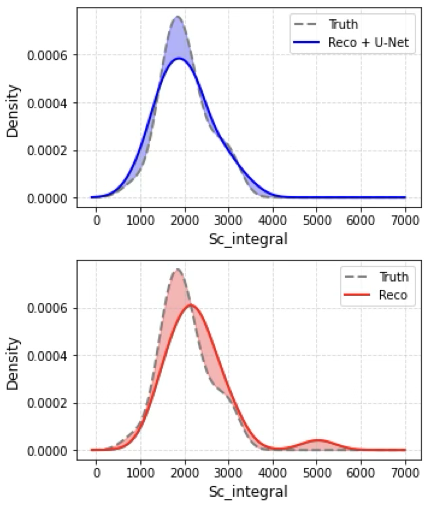
\includegraphics[width=\textwidth]{quali_images/1kev_result.png}
\caption{Distribuições de $S_c$ para eventos de \textbf{1~keV}. Linha
superior: Reco + U-Net (azul) vs.\ \textit{ground truth} (tracejado). Linha
inferior: Reco original (vermelho) vs.\ \textit{ground truth} (tracejado).
O pipeline com U-Net reproduz fielmente a distribuição de referência para ER
e NR. O algoritmo original apresenta desvio sistemático e caudas longas.
Fonte: apresentação à colaboração CYGNO (2024).}
\label{fig:result_1kev}
\end{figure}

Para 1~keV, o pipeline Reco + U-Net produz distribuições de $S_c$ que se
sobrepõem quase perfeitamente ao \textit{ground truth} para ambos os tipos
de recuo (ER e NR). O algoritmo original, em contraste, apresenta distribuições
sistematicamente deslocadas — com picos deslocados e caudas para valores altos
de $S_c$, indicando que pixels de ruído são incorretamente incluídos nos
clusters, inflando a estimativa de energia.

\subsection{Eventos de 0,5~keV}

A Figura~\ref{fig:result_05kev} apresenta os resultados para 0,5~keV, energia
em que a razão sinal-ruído é substancialmente menor.

\begin{figure}[H]
\centering
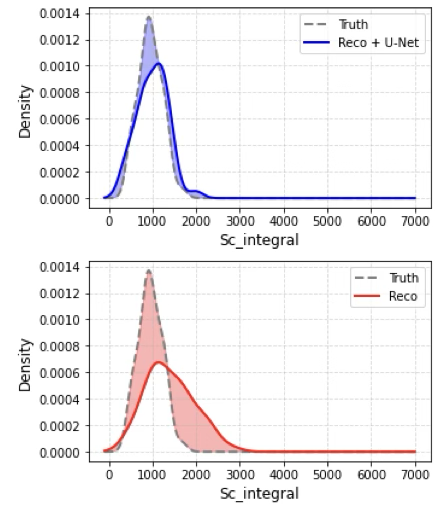
\includegraphics[width=\textwidth]{quali_images/05kev_result.png}
\caption{Distribuições de $S_c$ para eventos de \textbf{0,5~keV}. A degradação
do algoritmo original é mais acentuada que em 1~keV. O pipeline com U-Net
mantém as distribuições próximas ao \textit{ground truth}, demonstrando
robustez na redução da razão sinal-ruído. Fonte: apresentação à colaboração
CYGNO (2024).}
\label{fig:result_05kev}
\end{figure}

Com a redução de energia de 1 para 0,5~keV, observa-se que:
\begin{itemize}
    \item O \textbf{pipeline Reco + U-Net} mantém a concordância com o
    \textit{ground truth}, embora com um leve alargamento das distribuições
    — esperado, dado que o sinal é mais tênue;
    \item O \textbf{algoritmo original} apresenta degradação acentuada: as
    distribuições deslocam-se ainda mais, com sobreposição significativa
    entre os valores de $S_c$ de sinal e de ruído.
\end{itemize}

\subsection{Eventos de 0,25~keV}

A Figura~\ref{fig:result_025kev} mostra os resultados para 0,25~keV — a
energia mais baixa avaliada e o cenário mais desafiador, onde o sinal dos
pixels é praticamente indistinguível do ruído eletrônico.

\begin{figure}[H]
\centering
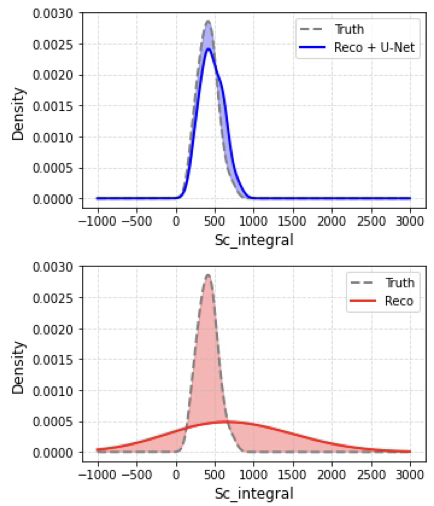
\includegraphics[width=\textwidth]{quali_images/025kev_result.png}
\caption{Distribuições de $S_c$ para eventos de \textbf{0,25~keV} — a energia
mais baixa avaliada. Mesmo neste regime extremo, o pipeline com U-Net
preserva distribuições próximas ao \textit{ground truth}. O algoritmo original
apresenta distribuições completamente desviadas, demonstrando incapacidade de
reconstruir a energia nesta faixa. Fonte: apresentação à colaboração CYGNO
(2024).}
\label{fig:result_025kev}
\end{figure}

Este é o resultado mais significativo deste trabalho: para eventos de
0,25~keV — exatamente a faixa de máximo interesse para WIMPs leves — a U-Net
ainda preserva uma estimativa de energia razoável. O algoritmo original, por
outro lado, apresenta distribuições completamente desviadas, sem nenhuma
correspondência com o \textit{ground truth}. Isso confirma que a limiarização
por $n \cdot \sigma$ é fundamentalmente inadequada para esta faixa de energia,
enquanto a U-Net, treinada com a Focal Loss, consegue identificar os pixels
de sinal mesmo quando suas intensidades são comparáveis ao ruído.

\subsection{Análise Consolidada}

A análise conjunta das três energias revela uma tendência clara: à medida que
a energia diminui de 1 para 0,25~keV, o desempenho do algoritmo original
degrada-se progressivamente, enquanto a U-Net mantém sua capacidade de estimar
a energia com precisão. Esse comportamento é consequência direta da
abordagem: enquanto a limiarização por $n \cdot \sigma$ aplica um critério
\textit{fixo} e \textit{local} a cada pixel, a U-Net aprende representações
\textit{contextuais} que levam em conta a vizinhança do pixel — reconhecendo
padrões espaciais de deposição de energia que se distinguem dos padrões
aleatórios do ruído, mesmo quando as intensidades individuais são comparáveis.

A Tabela~\ref{tab:summary_results} sumariza os principais resultados
quantitativos para toda a faixa de energia avaliada.

\begin{table}[H]
\centering
\caption{Resumo dos resultados do pipeline Reco + U-Net em comparação com o
algoritmo original (Reco), para eventos na faixa de 0,25 a 1~keV.}
\label{tab:summary_results}
\begin{tabular}{p{6cm}cc}
\toprule
\textbf{Métrica} & \textbf{Reco + U-Net} & \textbf{Reco (original)} \\
\midrule
Taxa de detecção verdadeira     & ${\sim}99\%$                      & Limitada            \\
Pixels ao iDBSCAN (por imagem)  & ${\sim}450$                       & ${\sim}50{.}000$    \\
Clusters falsos (mediana)       & ${\sim}3$--$4$                    & ${\sim}30$          \\
$S_c$ em 1~keV                  & $\approx$ \textit{ground truth}   & Desvio moderado     \\
$S_c$ em 0,5~keV                & $\approx$ \textit{ground truth}   & Desvio acentuado    \\
$S_c$ em 0,25~keV               & $\approx$ \textit{ground truth}   & Sem correspondência \\
Tempo de processamento          & Reduzido (GPU)                    & ${\sim}10\times$ maior \\
\bottomrule
\end{tabular}
\fonte{Elaborado pelo autor. Dados da apresentação à colaboração CYGNO (2024).}
\end{table}

\section{Significado Físico dos Resultados}
\label{sec:discussion}

Os resultados apresentados neste capítulo têm implicações diretas para a
sensibilidade do Experimento CYGNO à detecção de matéria escura leve:

\begin{enumerate}
    \item \textbf{Extensão do limiar de energia}: a capacidade de reconstruir
    a energia de eventos de 0,25~keV com precisão abre uma janela de
    detecção que era inacessível ao algoritmo original. Para WIMPs com massa
    de ${\sim}1$~GeV/c$^2$, os recuos nucleares depositam energias
    tipicamente abaixo de 1~keV — exatamente a faixa em que a U-Net
    demonstrou desempenho superior;
    \item \textbf{Redução de fundo}: a diminuição de clusters falsos de
    ${\sim}30$ para ${\sim}3$--$4$ por imagem implica uma redução de
    fundo que melhora diretamente a razão sinal/fundo do experimento;
    \item \textbf{Viabilidade operacional}: a redução do tempo de
    processamento por imagem torna viável o processamento em tempo quasi-real
    de grandes volumes de dados, requisito essencial para a operação
    contínua do detector nas fases futuras do experimento.
\end{enumerate}


%%==========================================================
\chapter{Conclusões e Próximos Passos}
\label{chap:conclusions}
%%==========================================================

\section{Retomada da Narrativa}
\label{sec:narrative}

Este trabalho é a continuação natural de uma linha de pesquisa. Na dissertação
de mestrado, demonstrou-se que técnicas de filtragem de imagens — especialmente
a rede neural U-Net — superam dramaticamente o algoritmo original do
Experimento CYGNO na seleção de pixels (F1-score: 0,873 vs.\ 0,137). O filtro
de mediana demonstrou ser uma alternativa computacionalmente eficiente
(4,3$\times$ mais rápido), capaz de reproduzir os mesmos resultados de energia
na análise de dados reais de $^{55}$Fe.

O passo seguinte natural era questionar: \textit{o quão longe vai a U-Net em
baixas energias?} O presente trabalho respondeu a essa pergunta com dados de
simulação na faixa de 0,25 a 1~keV — faixa de máximo interesse físico para
WIMPs leves, anteriormente inexplorada pelo grupo.

\section{Principais Resultados}
\label{sec:main_results}

Os resultados demonstram que a integração da U-Net ao pipeline de
reconstrução do CYGNO é altamente promissora:
\begin{enumerate}
    \item \textbf{99\% de taxa de detecção}: a U-Net detecta a esmagadora
    maioria dos eventos verdadeiros mesmo para eventos de 0,25~keV, onde o
    sinal é praticamente indistinguível do ruído eletrônico para métodos
    clássicos;
    \item \textbf{Estimativa de energia fiel}: a integral de cluster
    reconstruída pelo pipeline Reco + U-Net é próxima ao \textit{ground truth}
    para toda a faixa de 0,25 a 1~keV — resultado inatingível pelo algoritmo
    original;
    \item \textbf{Redução radical de pixels}: de ${\sim}50{.}000$ para
    ${\sim}450$ pixels enviados ao iDBSCAN por imagem (dois ordens de
    magnitude), com impacto direto no tempo de processamento;
    \item \textbf{Redução de eventos falsos}: de ${\sim}30$ para
    ${\sim}3$--$4$ clusters falsos por evento;
    \item \textbf{Focal Loss eficaz}: a adoção de $\alpha = 4$ demonstrou ser
    adequada para priorizar a revocação sem comprometer a precisão no regime
    de baixa energia.
\end{enumerate}

\section{Próximos Passos}
\label{sec:next_steps}

A partir dos resultados obtidos, três frentes de trabalho estão planejadas:

\subsection{Validação em Dados Reais}

O passo mais imediato é validar os resultados obtidos em simulação utilizando
dados reais do protótipo LEMOn. A principal dificuldade é a ausência de
\textit{ground truth} em dados reais; a estratégia proposta é utilizar fontes
radioativas de referência conhecidas (e.g., $^{55}$Fe a 5,9~keV;
$^{241}$Am) para verificar se as distribuições de energia reconstruídas pelo
pipeline Reco + U-Net são compatíveis com as esperadas. Comparações com
distribuições de Monte Carlo também serão realizadas.

\subsection{Robustez Frente a Variações no Perfil de Ruído}

O ruído eletrônico do detector pode variar com condições operacionais
(temperatura, tensão de alimentação, tempo de exposição e ageing do sensor).
Uma questão crítica é: o modelo U-Net treinado com ruído de um conjunto de
\textit{runs} específicos generaliza para \textit{runs} com perfis de ruído
diferentes?

A proposta é avaliar o desempenho do modelo frente a variações sistemáticas
do perfil de ruído, e, caso necessário, desenvolver estratégias de adaptação
de domínio ou retreinamento periódico com novos dados de ruído do detector.

\subsection{Exploração das Características da U-Net em Novas Aplicações}

Além da seleção de pixels, as representações intermediárias aprendidas pela
U-Net contêm informações ricas sobre os eventos. Três aplicações são
investigadas:
\begin{itemize}
    \item \textbf{Classificação ER vs.\ NR}: separação do tipo de recuo
    diretamente a partir da máscara gerada pela U-Net, sem necessidade de
    iDBSCAN — fundamental para rejeição de fundo no experimento;
    \item \textbf{Segmentação de instâncias}: identificação e separação de
    múltiplos eventos em uma mesma imagem, relevante para imagens adquiridas
    sem \textit{trigger};
    \item \textbf{Estimação direta de energia}: uso das características
    extraídas pela U-Net para estimar a energia sem o passo de agrupamento,
    eliminando a principal fonte de custo computacional do pipeline.
\end{itemize}

\section{Considerações Finais}
\label{sec:final}

O presente trabalho consolida a U-Net como a abordagem de referência para
seleção de pixels no Experimento CYGNO e estende sua aplicabilidade para a
faixa de baixa energia de máximo interesse físico. Os resultados são
promissores e estabelecem uma base sólida para as próximas etapas do
doutorado.

A contribuição central deste trabalho é demonstrar que o aprendizado profundo
não é apenas uma alternativa computacionalmente vantajosa ao algoritmo clássico
do CYGNO, mas uma ferramenta capaz de abrir uma nova janela de sensibilidade
física para o experimento — permitindo a análise sistemática de eventos abaixo
de 1~keV que seriam inacessíveis ao algoritmo original. Isso representa um
passo concreto em direção à meta de longo prazo do CYGNO: a detecção direta de
matéria escura leve com massas na faixa de 1 a 10~GeV/c$^2$.

\section*{Agradecimentos}

Os autores agradecem às seguintes instituições pelo valioso trabalho
colaborativo: INFN-Roma\,I, Gran Sasso Science Institute L'Aquila,
Dipartimento di Fisica della Sapienza Università di Roma, INFN-LNF, Museo
Storico della Fisica e Centro Studi e Ricerche ``Enrico Fermi'' e ao
Programa de Pós-Graduação em Engenharia Elétrica da UFJF.


\postextual

\bibliographystyle{unsrt}
\bibliography{mybibliography.bib}


\begin{apendices}

\chapter{\apendseq Arquitetura da U-Net Utilizada}
\label{apend:unet}

A U-Net foi adaptada da arquitetura original~\cite{ronneberger2015u} para
acomodar imagens de $2048 \times 2048$ pixels. A arquitetura completa,
incluindo as dimensões de cada camada, é apresentada a seguir.

\includepdf[pages=-]{image_files/u-net.pdf}

\end{apendices}


\end{document}
